%% (Master) Thesis template
% Template version used: v1.4
%
% Largely adapted from Adrian Nievergelt's template for the ADPS
% (lecture notes) project.


%% We use the memoir class because it offers a many easy to use features.
\documentclass[11pt,a4paper,titlepage]{report}

%% Packages
%% ========

%% LaTeX Font encoding -- DO NOT CHANGE
\usepackage[OT1]{fontenc}

%% Babel provides support for languages.  'english' uses British
%% English hyphenation and text snippets like "Figure" and
%% "Theorem". Use the option 'ngerman' if your document is in German.
%% Use 'american' for American English.  Note that if you change this,
%% the next LaTeX run may show spurious errors.  Simply run it again.
%% If they persist, remove the .aux file and try again.
\usepackage[english]{babel}

%% Input encoding 'utf8'. In some cases you might need 'utf8x' for
%% extra symbols. Not all editors, especially on Windows, are UTF-8
%% capable, so you may want to use 'latin1' instead.
\usepackage[utf8]{inputenc}

%% This changes default fonts for both text and math mode to use Herman Zapfs
%% excellent Palatino font. Do not change this.
\usepackage[sc]{mathpazo}

%% The AMS-LaTeX extensions for mathematical typesetting.  Do not
%% remove.
\usepackage{amsmath,amssymb,amsfonts,mathrsfs}

%% NTheorem is a reimplementation of the AMS Theorem package. This
%% will allow us to typeset theorems like examples, proofs and
%% similar.  Do not remove.
%% NOTE: Must be loaded AFTER amsmath, or the \qed placement will
%% break
\usepackage[amsmath,thmmarks]{ntheorem}

%% LaTeX' own graphics handling
\usepackage{graphicx}

%% We unfortunately need this for the Rules chapter.  Remove it
%% afterwards; or at least NEVER use its underlining features.
\usepackage{soul}

%% This allows you to add .pdf files. It is used to add the
%% declaration of originality.
\usepackage{pdfpages}
\usepackage{blindtext}

%% Make document internal hyperlinks wherever possible. (TOC, references)
%% This MUST be loaded after varioref, which is loaded in 'extrapackages'
%% above.  We just load it last to be safe.
\usepackage[linkcolor=black,colorlinks=true,citecolor=black,filecolor=black]{hyperref}


%% Document information
%% ====================

\title{Temporal Activity Detection in Untrimmed Videos with Recurrent Neural Networks}
\author{Alberto Montes}
% \thesistype{Final Degree Thesis}
% \advisors{Advisors: Xavier Gir\'o-i-Nieto, Amaia Salvador}
% \department{Imatge TSC ETSETB UPC}
\date{June 27th, 2016}

\begin{document}

%% Title page is autogenerated from document information above.  DO
%% NOT CHANGE.
\begin{titlepage}
    \maketitle
\end{titlepage}

%% The abstract of your thesis.  Edit the file as needed.
\pagenumbering{Roman}
\chapter*{Acknowledgements}
\pagenumbering{arabic}
First of all I would like to thank my two tutors of this project, Xavier Giró-i-Nieto and Amaia
Salvador for guiding and teaching me during all this project.

\chapter*{Abstract}

This thesis explore different approaches using Convolutional and Recurrent Neural Networks to classify and temporally localize activities on videos, furthermore an implementation to achieve it has been proposed.

As the first step, features have been extracted from video frames using an state of the art 3D Convolutional Neural Network. This features are fed in a recurrent neural network that solves the activity classification and temporally location tasks in a simple and flexible way.

Different architectures and configurations have been tested in order to achieve the best performance and learning of the video dataset provided. In addition it has been studied different kind of post processing over the trained network's output to achieve a better results on the temporally localization of activities on the videos.

The results provided by the neural network developed in this thesis have been submitted to the ActivityNet Challenge 2016 of the CVPR, achieving competitive results using a simple and flexible architecture.

\chapter*{Resumen}

Esta tesis explora diferentes enfoques usando Redes Neuronales Convolucionales y Redes Neuronales Recurrentes para clasificar y localizar temporalmente actividades en videos y propone una implementación propia.

Como primer paso, se han extraido descriptores de videos usando Redes Neuronales Convolucionales 3D del estado del arte. Estos descriptores se introducen en una Red Neuronal Recurrente que resuelve la clasificación de actvidades y su localización temporal de una manera simple y flexible.

Diferentes arquitecturas y configuraciones se han testeado con el objetivo de conseguir el mejor resultado y aprendizaje del conjunto de vídeos subministrado. Además, se han estudiado diferentes tipos de post procesado sobre la salida de la red entrenada para conseguir mejores resultados en la localización de actividades en los vídeos.

Los resultados obtenidos por la red neuronal desarrollada en esta tesis han sido publicados en la ActivityNet Challenge 2016 del CVPR consiguiendo resultados competitivos con una simple y flexible arquitectura.

\chapter*{Resum}

Aquesta tesis explora diferents enfocaments utilitzant Xarxes Neuronals Convolucionals i Xarxes Neuronals Recurrents per classificar i localitzar temporalment activitats en videos i proposa una implementació pròpia.

Com a primer pas, s'han extret descriptors de videos utilitzant Xarxes Neuronals Convolutionals 3D de l'estat de l'art. Aquests descriptors s'han introduït en una Xarxa Neuronal Recurren que resol la classificació d'activitats i la seva localització temporal d'una manera simple i flexible.

Diferents arquitectures i configuracions han estat testejades amb l'objectiu d'aconseguir el millor resultat i aprenentatge del conjunt de videos subministrats. A més, s'ha estudiat diferents tipus de post processat sobre la sortida de la xarxa entrenada per aconseguir els millors resultats en la localització d'activitats en els videos.

Els resultats obtinguts per la xarxa neuronal desenvolupada en aquesta tesis han estat publicats a la ActivityNet Challenge 2016 del CVPR aconseguint resultats competitius amb una simple i flexible arquitectura.


%% TOC with the proper setup, do not change.
\pagenumbering{arabic}
\tableofcontents
\listoffigures
\listoftables
\chapter{Introduction}

\section{Statement of Purpose}

Recognizing activities in videos has become a hot topic over the last years in the computer vision community~\cite{ngiam2011multimodal}. The exponential growth of portable video cameras and online multimedia repositories, as well as recent advances in video coding, storage and computational resources have motivated an intense research in the field towards new and more efficient solutions for organizing, understanding and retrieving video content.

Deep learning techniques have recently become the new state of the art in many computer vision tasks, such as image and object recognition in still images. While successful methodologies have been presented for image understanding, video content still presents additional challenges (e.g. motion, temporal consistency, ...)  that often cannot be bridged with still image recognition solutions.  

The purpose of this work is to address the challenges of video content analysis taking advantage of state-of-the-art deep learning techniques. The aim of this project is to develop a competitive framework to both classify and temporally localize activities on videos. To achieve this goal, the dataset used to fulfill this task is be the ActivityNet dataset \cite{caba2015activitynet}, which offers untrimmed videos depicting a diversity of human activities.

%Rather than focusing on activity classification on videos, the aim of this project is to offer a good framework to detect and localize activities on videos. To achieve this goal, the dataset used to fulfill this task will be the ActivityNet dataset \cite{caba2015activitynet}, which offers untrimmed videos which a huge variety of activities on it.

% AMAIA: I think that it is fine to say that you will both address activity classification and detection in your thesis, not just detection... DONE

In particular, this project's main contributions are:
\begin{itemize}
	\item The design and training of a deep learning model architecture, which is based on 3D Convolutional features and Recurrent Neural Networks.
    \item The development and analysis of post processing techniques for classification and temporal localization
    \item The release of an open sourced package containing all the tools to reproduce the experiments, as well as the conversion of a state-of-the-art C3D model from Caffe to Keras.
    
% REMOVED:    \item A framework to classify and localize activities on videos using deep learning techniques, more precisely using recurrent neural networks.
%    \item Develop techniques to process sequence output from Recurrent Neural Networks, to get the activities' localization on videos.
%    \item Explore different configurations of Neural Networks to achieve the best results in activity classification and detection.
%    \item Contribute to the research community porting a model to extract features from video from one deep learning framework to another and open sourcing the code.
\end{itemize}

% AMAIA: I am not sure whether these are your contributions or a summary list of everything you did in the thesis. For contributions, I would stick to:
% 1) The design and training of the architecture, which is based on 3D conv features and RNNs
% 2) The development & analysis of postprocesssing techniques for classification & detection
% 3) The release of an opensourced package containing all the tools to reproduce the experiments, as well as the conversion of a state-of-the-art 3CD model from Caffe to Keras.

This project has been developed at the \textit{Image Processing Group (GPI) of the Universitat Politecnica de Catalunya (UPC)} during the Spring 2016 semester. This group had already work in deep learning techniques for still images, but never before in video analytics. %In this sense, this is a pioneering work that sets a baseline technique and software for future research within the group. 
%REMOVED: This project has no baseline and all the code and development of deep learning techniques applied to video has been done from scratch.
% AMAIA: What do you mean with this sentence? I guess this is assumed in all projects unless stated otherwise... ALBERTO: I tried to say that it has all been done from scratch with no previous work on this field on the Image group.

\section{Requirements and Specifications}

This project has been developed with the implicit goal of seeting a baseline for video analytics with deep learning in the research group, so that future students and researchers to keep working on it. The requirements of this project are the following:
\begin{itemize}
    \item Design and train a deep neural network to classify and temporally localize activities on videos using the ActivityNet Dataset.
    \item Participate in the ActivityNet Challenge 2016, organized as a workshop in the top conference IEEE Conference on Computer Vision and Pattern Recognition (h5-index = 128).
\end{itemize}

% AMAIA: I guess that by requirements you mean "what you were asked to do/what we agreed to do" at the beginning of the project? I slightly modified it, uut feel free to add more items.

As this project has been developed from scratch, no prior specifications were defined. The specifications were decided taking into account the needs for the project and the available resources. All the development was done on \textit{Python} using a very well-known framework which is \textit{Keras}, also a pioneering use of this library in GPI. This Deep Learning wrapper facilitates the design and training of models over two computational frameworks: \textit{Theano}\cite{theano2016theano} and \textit{TensorFlow}\cite{abadi2016tensorflow}. Both  projects support complex and high demanding computations over both CPU and GPU. For this project \textit{Theano} was used as backend because, at the time of developing this project, it was the only one that had implemented the convolution 3D and max pooling 3D operations required for its development.

In addition to the software, specific hardware was required. The high demanding computational resources needed to train neural networks required the use of GPUs provided by the \textit{Image Processing Group} at UPC.

%DELETED: For the development of Deep Learning models and to do all the computations were used some frameworks in \textit{Python}. Because this project has been developed without a baseline, no prior specifications were required. Anyway, for the development of this project it has been decided to work with \textit{Python} for development and \textit{Keras} over \textit{Theano}\cite{theano2016theano} as the deep learning framework to use.

% AMAIA: "Anyway" is too informal...
% AMAIA: I don't know if this applies here, but what about the GPUs that you used? ALBERTO: I've just added

\section{Methods and Procedures}

\textcolor{red}{XAVI: I guess you do not know what to write here, is that right ? \\ALBERTO: Right. \\XAVI: I suggest you always follow as a guideline Andrea Calafell's thesis. Here, she offered a summary of her work. You could do the same, by just copying here part of the Abstract you wrote in the working notes. Check Andrea's thesis here: https://imatge.upc.edu/web/publications/fine-tuning-convolutional-network-cultural-event-recognition}

\section{Work Plan}

This project was planned to follow the packages detailed on this section, with the exception of some minor deviations described in Section~\ref{section:work_plan_deviations}.

\subsection{Work Packages}

\begin{itemize}
    \item WP 1: Project Documentation
    \item WP 2: Research for the State of the Art
    \item WP 3: Dataset to work with
    \item WP 4: Software to use
    \item WP 5: Experimentation and Results Evaluation
    \item WP 6: ActivityNet Challenge 2016 Participation
    \item WP 7: Delivery and Exposition of this project
\end{itemize}

\subsection{Gantt Diagram}

The Gantt diagram of this project's work plan can be found on the Figure~\ref{fig:gantt_diagram}.

\begin{figure}[H]
\begin{center}
% Em falta fer-lo 
%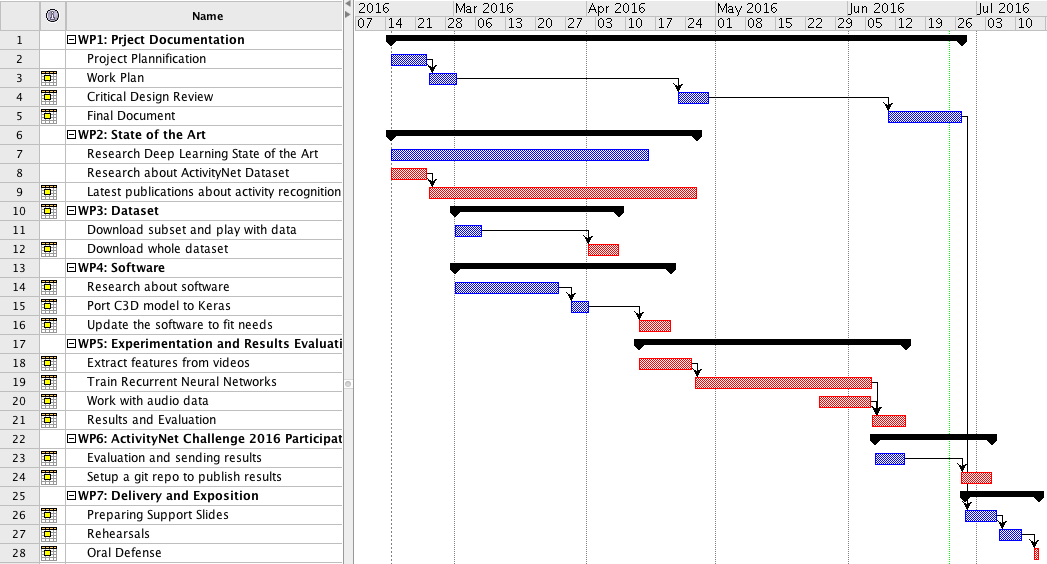
\includegraphics[width=1\linewidth]{img/introduction/gantt_diagram}
\end{center}
\caption{Gantt diagram of this thesis.}
\label{fig:gantt_diagram}
\end{figure}

\textcolor{red}{XAVI: Do not forget your Gannt diagram. You can always check the meetings notes I took if you do not remeber the exact timing of each task. This document should help you in revieweing everything you have been doing since February.}


\section{Work Plan Deviations and Incidents}
\label{section:work_plan_deviations}

The initial plan was to adapt the C3D\cite{tran2014learning} model for the ActivityNet task, which is implemented with the  \textit{Caffe} deep learning framework. But in order to use Recurrent Neural Networks, \textit{Keras} was a much better and flexible framework, so it was necessary to export the original C3D model from the Caffe framework to Keras.

Another deviation for the plan was that, due to the huge amount of required computational resources, fine tuning the full C3D network was not been possible. Instead, the C3D framework was used to extract features from the videos, which were later used as inputs to train the recurrent neural network.

Finally, the original work plan was extended by exploring the potential of audio descriptors for activity recognition. For this task, this work was supported by Professor Ignasi Esquerra from the TALP research group at UPC. He took care of extracting the audio features, which were later assessed and fused with the visual ones.

\chapter{State of the Art}

Over the last years deep learning techniques have evolved and have achieved incredible results for impressive tasks.
%AMAIA: I feel the message you are trying to give in this sentence is too broad ...? I think you can jump straight ahead to talk about deep learning solutions for video.

% AMAIA: For the state of the art, I think that you should re-organize it to cover the main different challenges of video analysis, and explain what people do to tackle each (even though you end up citing the same paper more than once in the process). You should also explain what you do in your project, and how it resembles or differs from what others did.

% 1. How do people use information in different frames? Some use 2D convolutions and merge them somehow, others use 3D conv. Here you can talk about pretrained networks (some people use VGG imagenet, there's people who have trained other models for Sports1M, right?)
% 2. How is motion encoded ? Some works directly use optical flow, while others directly input the visual data.
% 3. How do people ensure temporal consistency? LSTMs or GRUs
% 4. Particularly for activity detection, how do people do this? I remember the paper from columbia, where there are several stages. Maybe a strength of your work is that you train a single network that does it all (you just postprocess the output).
% ...


Many works in the literature have explored activity and action recognition problems using deep learning strategies. Most of them can be classified by the deep learning techniques used. Most of them used an approach of two stages (encoder and decoder) to learn from video's dataset. The first stage, the one being consider a decoder, is the stage that tries to encode the visual and temporal information from the input videos into some features vectors or information. The second stage, also known as decoder, tries from the extracted encoded information from the first stage, make a prediction of the output, which can be a classification of the video or a temporal localization of an activity.

Is very common see that as encoder, use Convolutional Neural Networks (or also known as CNNs) as it has been widely demonstrated that applying CNN networks to images and videos has obtain very good results in classifications tasks. A very well known and used CNN network is the VGG\cite{Simonyan14c} network which was top scored on ImageNet Challenge in 2014 on classification task. This network uses 2D convolutional kernels to extract spatial correlations from images and therefor learn how to classify them. Applying this techniques to activity detection, there are some implementations\cite{simonyan2014two}\cite{yeung2015every}\cite{Ng_2015_CVPR}\cite{ballas2015delving} using mostly the VGG network to encode video information.

% AMAIA: I think it's a good idea to cover the cited works in more detail. What are their differences? What do they have in common? Do you take ideas from them? What are the differences between what they do and what you do?

On the other hand very recently was proposed a CNN which tries to exploit both spatial and temporal correlations in video data using the additional dimension that videos offer and images do not. This is the 3D convolutional network, also referenced as C3D\cite{tran2014learning}. This network uses 3D kernels rather than 2D to extract videos information and try to learn from them. It has been widely used\cite{baccouche2011sequential}\cite{tran2015deep}\cite{tran2014learning}\cite{shoutemporal} for applications such as video classification. On some other research papers\cite{Yao_2015_ICCV}\cite{zhang2016modelling} the both approaches have been tried using 2D and 3D convolutional networks.

For this network, the input data is very common to use the raw video and let the network learn and extract information. Feeding the network with all the pixels of each frame in bunches of frames (the C3D is fed up with a 16 frame video clip) is very common, but in other cases some tricks are done. To feed up 2D convolutional layers but trying to learn from temporal correlations, what is done is compute the optical vector between frames and give it to a 2D CNN for training in combination with a parallel CNN fed up with the raw frames\cite{Ng_2015_CVPR}\cite{Yao_2015_ICCV}.

% AMAIA: "Bunches", "fed up", too informal...

%%%% Comments
Now talk about the recurrent neural network architecture proposed in the different papers of the state of the art. Talk about what RNN and LSTM are, some equations?

% AMAIA: Don't use equations in the state of the art. Maybe later in the methodology

Talk about some architectures interesting in the activity detection field and explain them more detailed (not much detailed but a little)??

% AMAIA: Yes, definitely ! I think that what you will explain in later sections is primarily focused on detection, so it is relevant that you explain what people have done in the past, and how your approach differs from them. I think what is interesting in your work is that you don't train in several stages using segment candidates. You train a single network. Ok, it does not improve the results, but the approach is much nicer ideally. 

\chapter{Methodology}

This chapter describes the required steps to achieve a functional deep neural network capable of detecting and classifying human activities in untrimmed videos. %For this challenge there was no baseline because video tasks have not been faced on the group I did this project, so was required to face the challenge from scratch.

% AMAIA: Again I think that it is assumed that you did all the work explained in this project.

\section{Objective}

The aim of this project is to design and train a deep neural network to classify and temporally localize activities in videos. The network is designed to exploit temporal information by combining Convolutional Neural Networks (CNNs) and Recurrent Neural Networks (RNNs). Short-term temporal information is captured by the 3D convolutional features computed over short video clips of 16 frames.
These features are later fed into a RNN that aims at recognizing longer-term temporal patterns. The RNN is expected to output a label for each clip of 16 video frames, preserving temporal consistency between close predictions in the output sequence. The design of the network enables both activity classification and detection capabilities using simple post-processing techniques on its output.

% AMAIA: I have changed this a bit. I think that all claims & comparison with other works should be done in the state of the art, results and conclusion sections. Here you should just explain your work.

%In order to get that, the proposal is, once the features have been extracted with the C3D, predict with a RNN a sequence of activities that might be happening for every 16-frame clip. So as the output of the Neural Network, is expected to have a sequence each item giving the activity happening at each video clip as input. This approach offers more advantages that others being able to classify the whole video and even localize along the video sequence them multiple activities happening and their temporal localization.

\section{ActivityNet Dataset}

Our model was trained and tested with the ActivityNet Dataset~\cite{caba2015activitynet}, a large-scale video benchmark for human activity understanding. This dataset (on its version 1.3, used in our work), contains 19,994 videos with different 200 activities labeled, representing a wide range of human activities. While this large dataset allows training the millions of parameters that define a neural network, it also poses important computational challenges due to the high performance computing and storage it requires.

\begin{figure}[t]
\begin{center}
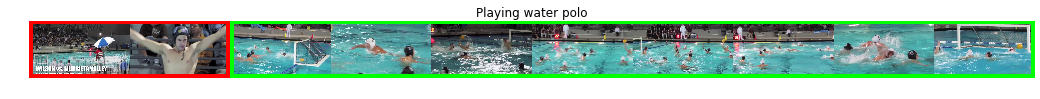
\includegraphics[width=1\linewidth]{img/methodology/activitynet_examples/activitynet_example_1}
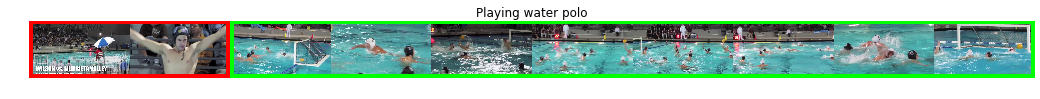
\includegraphics[width=1\linewidth]{img/methodology/activitynet_examples/activitynet_example_2}
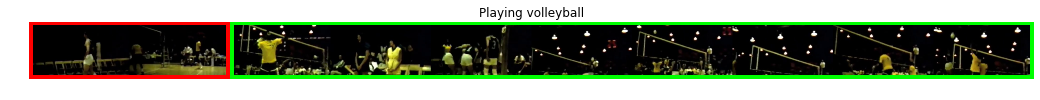
\includegraphics[width=1\linewidth]{img/methodology/activitynet_examples/activitynet_example_3}
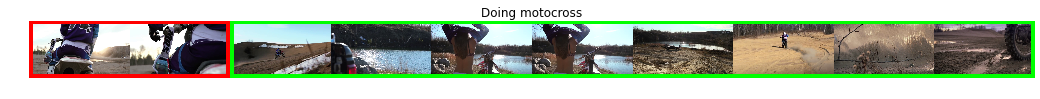
\includegraphics[width=1\linewidth]{img/methodology/activitynet_examples/activitynet_example_4}
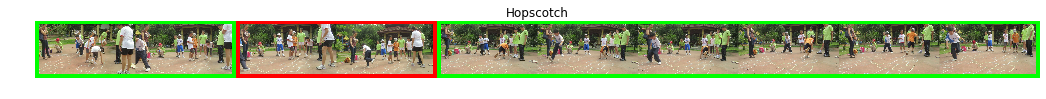
\includegraphics[width=1\linewidth]{img/methodology/activitynet_examples/activitynet_example_5}
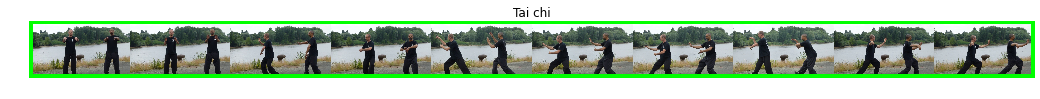
\includegraphics[width=1\linewidth]{img/methodology/activitynet_examples/activitynet_example_6}
\end{center}
\caption{Sample of videos from the ActivityNet Dataset}
\label{fig:dataset_example}
\end{figure}
% AMAIA: I think this section is asking for a figure with some examples of the dataset :). Maybe they have a figure like this in the website or their paper already? ALBERTO: DONE

ActivityNet 1.3 contains 660 hours of video, which are split in the following way: 50\% training set, 25\% validation set and 25\% testing set. Each video of the dataset is annotated with a single activity, along with all temporal locations in which the activity occurs. Figure~\ref{fig:dataset_example} presents examples of videos of different activities and its temporal annotations.

The dataset is provided as a description text file, with the URL of the video and also the ground truth annotations, as the starting time, ending time and the class of activity in the  given interval. In addition, the original video resolution and the duration are also provided.

Because all the videos from this dataset are hosted on \textit{YouTube}, only their links are provided to avoid copyright issues. For this reason, the first and costly task was downloading all the videos from their URLs. This was done using a library called \textit{youtube-dl}\footnote{\url{https://rg3.github.io/youtube-dl/}}, which allows downloading YouTube videos with Python calls. Some issues arose during the acquisition of the dataset, such as videos being removed by their owners, or being blocked due to localization restrictions. In those cases, videos could not be downloaded and therefore were not used in the experiments. The total size of the used dataset was of 19,811 videos.

% AMAIA: I changed some of the text above to be less informal in general... but you should try to do it from this point on.

Once the videos from the dataset were downloaded, the number of frames of each video was also computed to be able to convert from seconds to frames in the temporal domain.
% AMAIA: I don't understand what you mean in the above text. I guess you want to say that all frames from all videos are used ( no subsampling)? The resolution part I don't get. In any case, this does not belong in this section. You should explain this when you talk about feature extraction.
% ALBERTO: ok done
In addition, other stats were computed, such as the whole number of frames from all the videos in the dataset, which is 65.6 million frames. Also, the length in minutes of each activity at the dataset was plot on Figure~\ref{fig:dataset_stats}, to have an estimation about the activities duration. As it can be observed, not all the activities have the same duration along the dataset, varying from 40 minutes as the total activity duration
%\textcolor{red}{XAVI: what do you mean by the total activity appearance ? Is it the average length ? ALBERTO: No. Is the total length of the annotations of each activity}
to 3.5 hours for the longest activity. In total, over all the dataset there are 313 hours of activities which needed to be detected and classified in the 660 hours of video.

\begin{figure}[ht]
\begin{center}
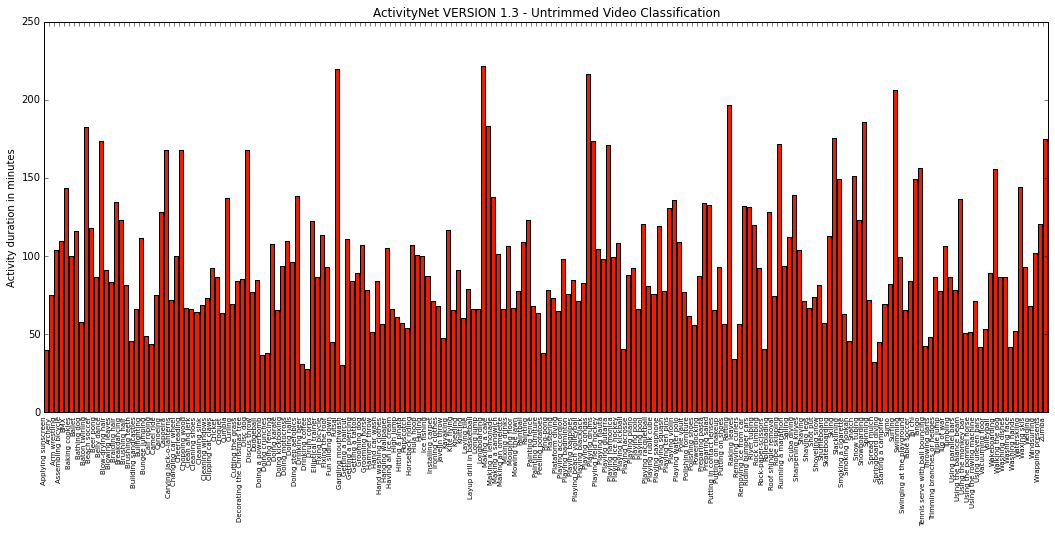
\includegraphics[width=1\linewidth]{img/methodology/dataset_stats}
\end{center}
\caption{Activity duration in minutes for each activity in the dataset}
\label{fig:dataset_stats}
\end{figure}

\section{Extraction of Video Features Using C3D}

The C3D network~\cite{tran2014learning} was chosen as a feature extractor, due to its good performance in previous works~\cite{baccouche2011sequential,tran2015deep,tran2014learning,shoutemporal}. This network is composed of 8 convolutional layers, plus 5 pooling layers, 2 fully-connected layers and a Softmax output at the end.
The convolutional layers have $3 \times 3 \times 3$\footnote{For notation, the dimension ordering is $d \times k \times k$ where $d$ is temporal dimension and $k$ is spatial dimension} kernels and stride 1 while at the same time the pooling layers compute the maximum at every kernel size of $2 \times 2 \times 2$ (except from the first pooling layer which has a $1 \times 2 \times 2$ kernel size).
The two full-connected layers (\textit{fc6} and \textit{fc7}) have both 4096 neurons while the Softmax output has 200 outputs as the number of classes of the Sports1M Dataset. Figure~\ref{fig:c3d_architecture} shows a representation of the C3D architecture, including the number of kernels or neurons of each convolutional layer and fully-connected layer respectively.

\begin{figure}[H]
\begin{center}
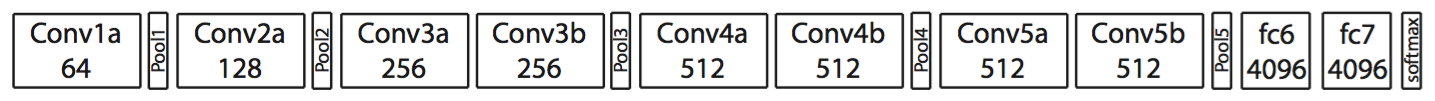
\includegraphics[width=1\linewidth]{img/methodology/c3d_architecture}
\end{center}
\caption{The C3D Architecture}
\label{fig:c3d_architecture}
\end{figure}

The input of the network are clips of videos of 112x112 frames width and height and 16 frames of temporal depth. It was decided to extract the video features at the fully-connected layer \textit{fc6} because it has been reported to work well for both image classification tasks~\cite{girshick2014rich} and input feature for training a RNN~\cite{donahue2015long}.

The C3D model~\cite{tran2014learning} was developed over a version of \textit{Caffe}~\cite{jia2014caffe} dated in 2014. This version did not support the \textit{Python} environment used for this project, nor provides tools for implementing RNNs. Given the relevance of RNNs in this work, it was decided to move to the \textit{Keras} framework, which provided the required tools. As a consequence, the C3D model in Caffe trained with the Sports1M~\cite{KarpathyCVPR14} dataset, was ported to \textit{Keras}.
This was an unexpected contribution of this thesis, which was warmly received by the community of Keras developers. Its main contributor, François Chollet, tweeted about our ported model. All the process has been open sourced and is available online\footnote{ \url{https://gist.github.com/albertomontesg/d8b21a179c1e6cca0480ebdf292c34d2}}.

% AMAIA. Comments for the above text:
% 1. The sentence explaining what keras is should go someplace else (maybe in the requirements section ?) ALBERTO: Put on requirements.
% 2. I thought we did not use caffe because it does not support RNNs (at least not the 'vanilla' version right?) RIGHT

At the time to run the C3D model on the model ported to \textit{Keras}, some small changes were applied Keras' source code\footnote{The fork of \textit{Keras} used can be found in: \url{https://github.com/albertomontesg/keras/tree/improved-3d-ops}}, involving the implementation of the 3D convolution and 3D pooling operations. Once this was fixed, all the videos were forwarded through the C3D model, and the features from the first fully connected layer \textit{fc6} were extracted.
This process used 2 GPUs in parallel for feature extraction, and multiple CPU cores fetching all the videos from disk. The usage of 2 GPUs in parallel reduced the computational time expected for this task from 1 week to 2 days.

% AMAIA: I think that before the above paragraph you should say that you use 16-frame clips, and that you extract a fc6 for each of them. ALBERTO: I think that now done.

In the process of fetching the videos from disk, the \textit{OpenCV}~\cite{opencv_library} library was used. With this software, the videos were read in chunks of 16 frames, resized to 112x112 as input frame size, remove the mean for each color channel which the original model was trained with and then forwarded through the C3D network. The values of the model at the full-connected layer fc6, a sequence of 4096-sized vectors was stored in disk for preparing it to train the Recurrent Neural Network. % AMAIA: fc6 is not the output of the model, but the features that you chose to extract. ALBERTO: Change

\section{Extraction of Audio Features}

Audio features were also explored as potential sources of information to recognize the activity depicted in the videos. As previously explored for activity detection~\cite{xu2015uts}, some audio descriptors were extracted to improve the detection and classification results. In this project, the MFCC and Spectral descriptors were adopted~\cite{heittola2013context}.

Both MFCC and Spectral descriptors were extracted using specialized software: SPro~\cite{gravier2010spro} and Essentia~\cite{bogdanov2013essentia} respectively. For the MFCC descriptors, 40 values were extracted for 10ms temporal windows. Because the misalignment of scale between the features extracted for video and MFCC videos, the second ones were grouped to have the same sequence length of audio features and video features.

In order not to lose too much information when grouping the features, the mean and standard deviations along the temporal scale were computed, so at the end 80 values were available to represent the MFCC features from the audio video's track.

On the other hand, the Spectral features were extracted to have information about the energy distribution on the frequency domain along the video, so only 8 values were extracted for each videos. At the time to give the audio features at the input of the Recurrent Neural Network, for each video clip feature vector, it was concatenated the MFCC features grouped for the temporal window of the clip and then also concatenated the spectral features of the whole video the clip belong.

\section{Recurrent Neural Networks}

Recurrent Neural Networks (RNNs) were adopted as the basic module to solve the main task of this project. Among these family of deep learning architectures, the Long-Term Short Memory networks (LSTMs) were adopted thanks to their ability to learn long term correlations. %Different architectures were built and tested around these modules. %The RNN had the inputs and output previously explained, and so an experimentation of the architecture was done.

The basic architecture consist in a single layer of LSTM with 512 cells, which is defined with a total of 9.5 millions parameters. A more advanced architecture would consider two layers of LSTMs, as shown in  Figure~\ref{fig:lstm_architecture}.% there is represented the network architecture.

\begin{figure}[H]
\centering
\begin{subfigure}[b]{.5\textwidth}
  \centering
  \includegraphics[width=1\linewidth]{img/methodology/lstm_architecture_basic}
\end{subfigure}%
\begin{subfigure}[b]{.5\textwidth}
  \centering
  \includegraphics[width=1\linewidth]{img/methodology/lstm_architecture_deep}
\end{subfigure}
\caption{Architecture of RNN used with 512-LSTMs with one and two layers respectively.}
\label{fig:lstm_architecture}
\end{figure}

During the development of this work, it was observed that the single layer architecture provided very different classes in short periods of time, providing this way very inconsistent results. For this reason, a more sophisticated architecture was introduced, which inserted as
%With the basic architecture was observed that the activity prediction, in some cases was very different in short periods of time, predicting between two activities or one activity and the background class. To solve this problem, another architecture proposed consist in the previous basic one, but with
an additional input the activity predicted for the previous clip.
%at the bottom which consist the previous output of the sequence.
Figure~\ref{fig:lstm_architecture_feedback} presents this advanced architecture.
This new input with the information about the previous activity was
%codified in a one-hot encoding\footnote{One-hot encoding means to encode integer values into a vector of zeros and a single 1 on the position specified by the given value} and was expanded to have an extra class which will be given at the beginning of each video as it does not have previous output. This input was
fuse in a concatenation operation with the already extracted features vector and then used to train the Recurrent Neural Network. This kind of feedback on the Network was expected to give smoother predictions, as the network is aware about the previous activity.

%The previous activity encoded in a one-hot encoding\footnote{One-hot encoding means to encode integer values into a vector of zeros and a single 1 on the position specified by the given value} was concatenated to the current video features.  \textcolor{red}{XAVI: It is not clear to me how you combine the video features and this one-hot vector. Are they concatenated ? You seem to state that they are summed.
%Is this correct ? Please clarify}. which will be always zero except to the first video feature, which do not have previous output, and will be marked with a one. With this extra value, it is expected that the network learn to forget its memory state because the begging of a video sequence.  \textcolor{red}{XAVI: This is also confusing. First, you should explain what a one-hot encoding means. Later, I do not see the relationship between the feedback and making the network to forget. Please rephrase and explain better}. This kind of feedback, was expected to give smoother predictions, as the network is aware about the previous activity.
%can be found the architecture previously explained with feedback.

\begin{figure}[H]
\begin{center}
\includegraphics[width=0.6\linewidth]{img/methodology/lstm_architecture_feedback}
\end{center}
\caption{Architecture of the RNN network with feedback from the previous output}
\label{fig:lstm_architecture_feedback}
\end{figure}



%%%%% Talk about semisupervised training???????


\section{Data Preparation}

While training of neural networks, both the input and output data are grouped in batches to perform parallel and faster computations of the learning algorithm. This batches have all the same number of fixed length sequences of both inputs and outputs vectors of the dataset.
%and contains a multiple fixed \textcolor{red}{XAVI: multiple and fixed seem a bit contradictory... is this the right terminology ? Maybe you can rephrase this ?} length sequence of both inputs and outputs of the dataset.
The length of all the sequences given at each batch is called \textit{timestep} and must be a low value so that the gradient propagates along all the sequence. Otherwise the gradient might achieve very high values, a problem known as \textit{exploiting gradient}.

Most video datasets include content of different lengths, which forces a pre-processing to build training batches of a fixed length.
%Since in all major video datasets, videos are not from the same length, the videos data must be carefully prepared.
When training Recurrent Neural Networks, the internal state (which represent the memory stored) of the LSTMs is preserved for every batch computation but then reset between batches. As the sequences of features vectors extracted from videos in the dataset are longer the than the \textit{timestep} used, during training the memory state of the LSTMs will be reset multiple times (depends on the video length).

%It is required, if the goal is learn from long sequence data, as it is the videos of the dataset, to keep the memory of the LSTM alive for long sequences. \textcolor{red}{XAVI: You need to explain better this "LSTM alive" concept that you state. Be more rigurous and help the reader in understanding your text. Do not assume the reader is an expert on this topic. This will probably be the first time s/he reads about LSTMs and training DNN.}
% AMAIA: You should add a section explaining your architecture before you start talking about how to train it ! So basically section 3.6 should come before this one. ALBERTO:DONE

% AMAIA: A friendly intro explaining that  deep nets are usually trained on batches, which contain many samples of the dataset (of the same size)and are processed in parallel. The problem you have is that videos are too long and therefore do not fit in a single batch (risk of exploding gradients as well), so you need to cut them in pieces to separate them in different batches, and also make sure that LSTM memory is preserved from batch to batch.

% REMOVED: Since all the videos on the ActivityNet Dataset are not from the same length, to train a recurrent neural network, it requires to give it a fixed length sequence. This length is called \textit{timestep} and must be a value not very high because as the gradient propagates along all the sequence, if the timestep is very high, the gradient might achieve very high values known as \textit{exploiting gradient}.

There exist two solutions to this problem. The first solution is organizing data in batches of a large \textit{timestep}, but this would require to clip the gradients, as explained in~\cite{pascanu2012difficulty}. The second solution is to train the RNN without resetting the memory from batch to batch. With this approach, if a video sequence (Equations~\ref{eq:video_seq_1} and~\ref{eq:video_seq_2}) is longer than the \textit{timestep}, the RNN can be trained by passing fragments of the videos as clips, one after the other in different batches, but at the same batch position. Since the memory is not reset after each batch, the video sequence is processed smoothly.

\begin{equation}
	\bar{X} = [x_i, x_2, \ldots, x_{4096}]
    \label{eq:video_seq_1}
\end{equation}
\begin{equation}
	V_i = \{ \bar{X}_t \}_{t=1}^{T_i}
    \label{eq:video_seq_2}
\end{equation}

For this configuration, the different videos must be carefully set on the same batch index to exploit the \textit{Keras} functionality of \textit{stateful} training for RNNs. Figure~\ref{fig:stateful_dataset} depicts how the video features are organized to train the Recurrent Neural Network. The notation for the data is as follows: $\bar{X}$ is the feature vector of a 16 frame clip extracted from the C3D network, and $V_i$ the sequence of features for a single video. Note that $T_i$ is the length of the sequence of each video $i$ in number of 16-frame clips.

\begin{figure}[ht]
\begin{center}
\includegraphics[width=1\linewidth]{img/methodology/stateful_dataset}
\end{center}
\caption{Graphical representation of how the data is sorted in batches}
\label{fig:stateful_dataset}
\end{figure}


%In order to try to fit the most possible data into the GPUs when training each batch and to get a good gradient propagation along the batch's sequence length, for all the experiments done on this project, the batch size was 256 and the timesteps 20. % AMAIA: The values of this parameters should be given in the experiments section- % ALBERTO: Completely agree

As the last step to prepare the data, the misalignment between the blocks of 16 frames and the detailed annotation provided by the ground truth had to be considered. During our training, if the Intersection Over Union (IOU) between the 16-frame clips and the ground truth annotations was higher than $0.5$, the clip was considered as \textit{activity}. On the other hand, if the IOU was below $0.5$, the clip was considered as \textit{background (no activity)}. %\textcolor{red}{XAVI: The next sentences seem to express a completely different idea, right ? Should it be a different paragrpah ? I also wonder if this is something you alerady explained previously, a few paragrpahs earlier...}.

So at the training and validation subsets, the output was encoded with the one-hot encoding, which puts a 1 at the position of the class given and 0s on the rest.  This way to encode the output is the used for Softmax output layers which represent the probability of each class to be predicted as the output is between 0 and 1. The same codification was used on the network which feedback the previous output, but an additional class was added. For the first element of each video, as they do not have a previous output, a \textit{\textless START\textgreater} class flag was given.

% AMAIA: The above paragraph is explaining the evaluation of the output. This does not go here, but later in the experiments section. ALBERTO: NO, this is trying to explain how is set the output for training for each of the 16-frames clips. This is the step of how I pass from a list of temporal annotations to have some 16-frame clips with a class on each.
% AMAIA: Again, the explanation of how to encode class labels as one-hot vectors should come later. ALBERTO: This is how the output data is prepared. I think that may fit better on the methodology chapter.


\section{Training Methodology}
\label{section:training}
% ALBERTO: I'm aware that there are two sections call training both in methodology and results. May I change the name of this one??
% XAVI: Maybe you can call teh

During training, each batch is forwarded to the Neural Net and with the output predicted and the ground truth given, the loss is computed. The objective of every learning step is to reduce the loss, so using a specific gradient computation, the parameters of the network are updated in proportion of the computed gradient and a value previously set called the learning rate. As the training goes on, it is expected and required that the loss value after every batch decreases for both training and validation subsets. The first subset is the one used to update the model's parameters while the second one is used to test the behavior of the network while training.

It is very common that if the learning rate is not correctly set, the loss for the training set (the one the network learns from) goes down, while it increases for the validation set. This will mean that the network has only learned for the subset seen but the prediction over the rest of the dataset are not valid. This effect, which can be explained if the network has very high learning capacities, is called over-fitting and is undesirable. Also while training, the accuracy is tend to be computed to check that the accuracy of the prediction increases.

The training of RNNs allows learning the parameters that govern their behavior. The training process itself is also determined by certain design decisions.
Firstly, the loss function, also known as objective function, allows assessing the performance of the trained network by comparing its prediction over the training set. As the last layer used was a Softmax which is non-linear function that gives values between 0 and 1, the output can be understand as the probability of predicting each of the classes at the output. Having at the output a distribution of probability, the common computation of the loss is using the \textit{categorical cross entropy}.

The \textit{categorical cross entropy} function is described in Equation~\ref{eq:crossentropy} and represents the average number of bits needed to identify an event drawn from the set, if a coding scheme is used that is optimized for the predicted probability distribution $q$, rather than the ground truth probability distribution $p$. This function is higher as more different the predicted distribution and the ground truth are.%    We adopted the \textit{categorical cross entropy}, because the output of the softmax can be considered as a probability distribution. \textcolor{red}{XAVI: Could you develop a bit more ?}

\begin{equation}
\label{eq:crossentropy}
	H(p,q) = - \sum_x p(x) \log(q(x))
\end{equation}

Secondly, the learning rate controls how quickly the parameters of the model are updated.
Figure~\ref{fig:training_curves_comparison} shows the learning curves of the same network with a different values of learning rate. On this curves the loss (blue) and the accuracy (red) are plot over the epochs, and also separated by subset: training (thin line) and validation (striped line). Note that an epoch is the number of iterations required to have forwarded all the batches of the dataset once. In our case, the best learning rate was $10^{-5}$. %\textcolor{red}{XAVI: I think this is the first time you present these learning curves. You should describe them more to help the reader understaands the message. Again, please do not suppose your reader is an expert of deep learning, but somebody who is having his first contact with it.}

%paraotherwise, have been the value that has need to be tuned. At the training, starting with high values for the learning rate, it was observed that the network did not learned and the validation loss increased instead of decreasing.



\begin{figure}[H]
\centering
\begin{subfigure}[b]{.5\textwidth}
  \centering
  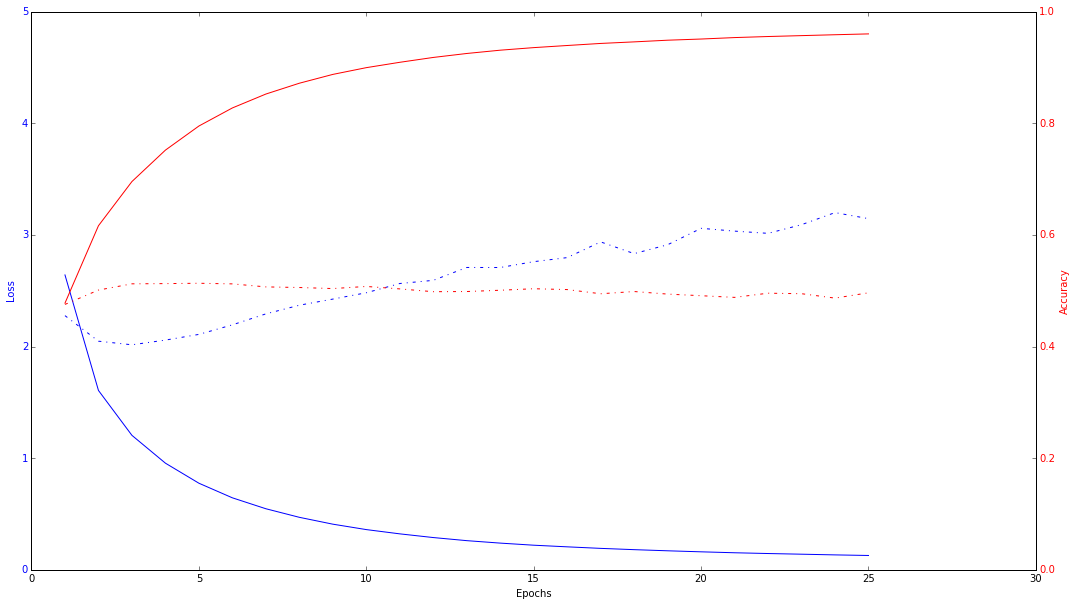
\includegraphics[width=1\linewidth]{img/methodology/training_bad}
\end{subfigure}%
\begin{subfigure}[b]{.5\textwidth}
  \centering
  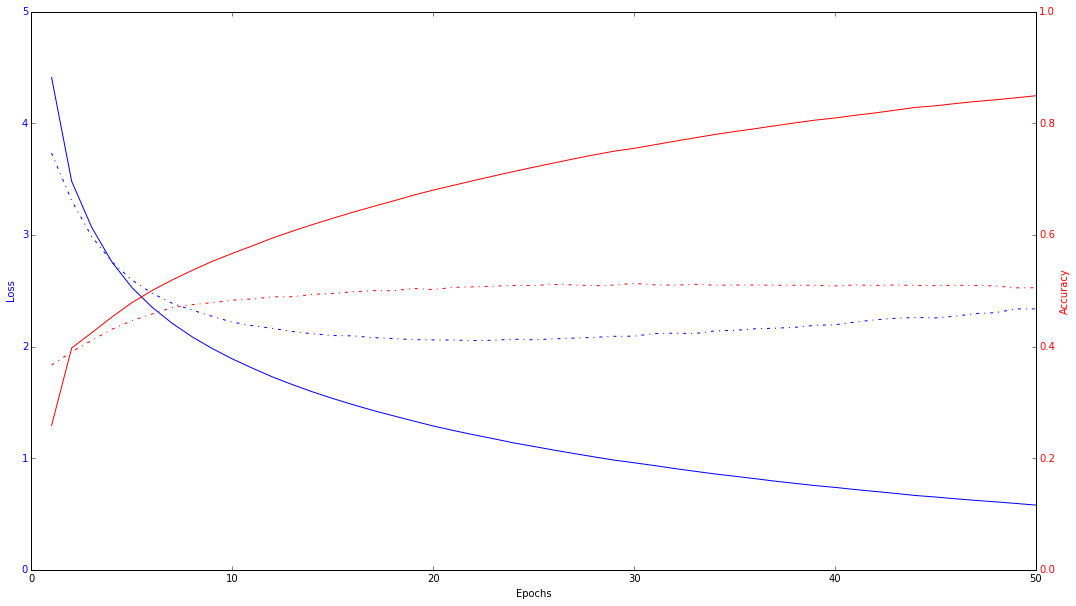
\includegraphics[width=1\linewidth]{img/methodology/training_good}
\end{subfigure}
\caption{Comparison of the learning curves. On the left with a learning of $10^{-4}$ and at the right figure with a learning rate of $10^{-5}$}
\label{fig:training_curves_comparison}
\end{figure}

It was observed that the network presented some over-fitting due mostly to the high learning capacity the network has over the data. %\textcolor{red}{XAVI: You should describe what is over-fitting and high learning capacity.}
This over-fitting problem can be addressed by adding dropout~\cite{srivastava2014dropout} layers before and after the LSTM layers. Dropout consists in randomly setting a fraction $p$ of input units to 0 at each update during training time. %The value of $p$ chosen was 0.5.

The combination of visual and audio features required a normalization step, as they presented different statistics and range of values.
%Another inconvenience found during training, was related to the fact of having as an input multiple vectors from multiple sources.
%When training with the visual features extracted from the C3D network, with the audio features or/and the previous output, as all of them presented a different statistics, a normalization was required.
So for all the experiments, a batch normalization~\cite{ioffe2015batch} was included after the input data in order to have all the inputs with the same statistics, mean 0 and standard deviation equal to 1.

The last problem that was necessary to face, was related to an unbalanced distribution of classes in the dataset. All the activities had approximately the same frequency of appearance, but nearly half of the video clips correspond to a non-activity, or as previously defined, background class.
Given the used categorical cross entropy as loss function, the network tended to predict the background class. For this reason, it was decided to weight the loss function in order to slow down the learning of weights when the background class was predicted. %With this method the predicted output will not be so bias towards the background class.

The weighted loss function taking into account the unbalanced classes is defined as

\begin{equation}
	H(p,q) = - \sum_x \alpha(x) p(x) \log (q(x)), \text{ where } \alpha(x) =
    \begin{cases}
        \rho, & x = \text{background instance}\\
        1,    & \text{otherwise}
    \end{cases}
\end{equation}

where $\rho$ is the factor used to weight the loss for background instances at training. This value $\rho$ is usually computed as 1 minus the frequency of appearance of the class (for all the activities class can be simplified to 1). %For the background class was found the its frequency of appearance was 0.4 so it was tested to setup $\rho = 0.6$. The results did present a little improvement so it was decided to even do smaller this value, setting it finally $\rho = 0.3$.

\section{Post-Processing}
\label{section:post_processing}

The proposed network generates as an output the predicted activity probability for each 16-frames clip.
These clip-wise predictions were post-processed to solve the project goals of activity classification and detection.

%For the challenge to face during this project, and for the aim of this project is required to compute from the output obtained the activity classification for the whole video and the temporal localization of this activity. To obtain this information, some post-processing was required as it is not directly predicted from the network.

\subsection{Classification Task}

For the classification task, the first step was removing the output probability corresponding to the background class, as it is known that all videos in the ActivityNet Dataset depict one, and only one, activity. Once the background class was removed, then the mean of each video activity class was computed along the video's output sequence.

\begin{equation}
	p_{video}(x) = \frac{1}{T_{video}} \sum_i^{video} p_i(x), \text{where } x \in \{ \text{Dataset Activities}\}
\end{equation}

With this operation, each video in the dataset is associated to a vector of probabilities, each one giving the probability of each activity happening along the video. The classification task was solved by selecting the activity with the highest probability.

\subsection{Detection Task}

For the detection task of the ActivityNet Challenge, also referred as temporal activity localization, more operations were required. We exploited the fact that each video in ActivityNet dataset is annotated with a single activity class, which may occur at multiple temporal segments. % is known that at every video of the ActivityNet Dataset all the annotation are of the same activity, the classification activity was first computed and give it as solution for all the temporal localization.

The sequence probabilities predicted by the RNN were filtered with the \textit{mean} operator of size $k$, being $k$ the size of the window backwards and forward. Equation~\ref{eq:mean_filter} defines this filter. This filtering step generated a smoother output prediction.

\begin{equation}
	\tilde{p}_i(x) = \frac{1}{2k} \sum_{j=i-k}^{i+k} p_i(x)
    \label{eq:mean_filter}
\end{equation}

The next step was for every step of the output sequence, compute the activity probability as the sum of all the output classes except the background class.
\begin{equation}
	\tilde{p}^a_i = \sum_{x=1}^{200}\tilde{p}_i(x), \text{where } x = \begin{cases}
        0, & \text{background class} \\
        i, & 1 \leq i \leq 200 \text{ activity classes}
    \end{cases}
\end{equation}

%\textcolor{red}{XAVI: Should not this Equation 3.7 be the same as 3.5 ? ALBERTO: NO. in 3.5 it is computed the mean along the sequence, and in 3.7 it is sum the probability of having an activity at each step of the sequence.}

Finally, only those activity detection with $\tilde{p}^a_i$ over a certain probability threshold ~$\gamma$ were considered. The rest were discarded as they did not meet a minimum of confidence. Both parameters $k$ and $\gamma$ were learned also during the training process described in Section~\ref{section:results}

%In particular, those detections with an activity probability $\tilde{p}^a_i$ higher than the threshold $\gamma$. Playing with the values of $k$ of the mean filter and the threshold $\gamma$ it has been possible to find the best values to get the best performance. The results of all the experimentation described on this section is detailed on Section~\ref{section:results}

\chapter{Results}
\label{section:results}

On this section, the results of the multiple experimentation will be given and detailed.

\section{ActivityNet Dataset}

The ActivityNet Dataset\cite{caba2015activitynet} is \textit{A Large-Scale Video Benchmark for
Human Activity Understanding}. This dataset (on its version 1.3, the one used for the challenge), contains 19,994 videos with different 200 activities labeled, representing a wide range of human activities. 

\begin{figure}[t]
\begin{center}
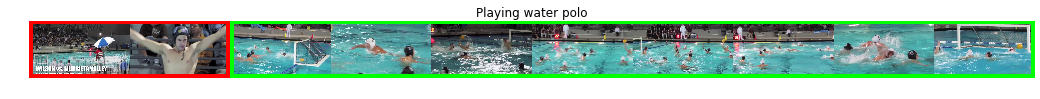
\includegraphics[width=1\linewidth]{img/methodology/activitynet_examples/activitynet_example_1}
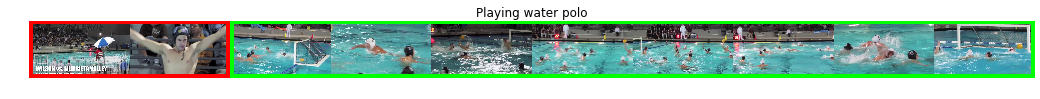
\includegraphics[width=1\linewidth]{img/methodology/activitynet_examples/activitynet_example_2}
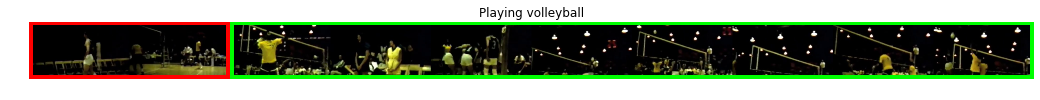
\includegraphics[width=1\linewidth]{img/methodology/activitynet_examples/activitynet_example_3}
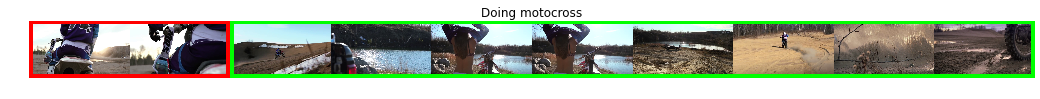
\includegraphics[width=1\linewidth]{img/methodology/activitynet_examples/activitynet_example_4}
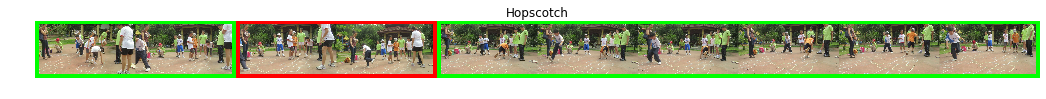
\includegraphics[width=1\linewidth]{img/methodology/activitynet_examples/activitynet_example_5}
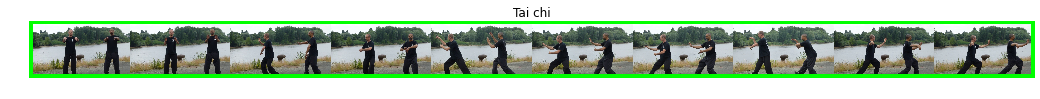
\includegraphics[width=1\linewidth]{img/methodology/activitynet_examples/activitynet_example_6}
\end{center}
\caption{Sample of videos from the ActivityNet Dataset}
\label{fig:dataset_example}
\end{figure}
% AMAIA: I think this section is asking for a figure with some examples of the dataset :). Maybe they have a figure like this in the website or their paper already? ALBERTO: DONE

In total there are 660 hours of video and the subsets are split in the following way: 50\% training set, 25\% validation set and 25\% testing set. Each video of the dataset is annotated with a single activity along with the annotation of all temporal locations in which the activity occurs. On the Figure~\ref{fig:dataset_example} there is examples of videos of different activities and its temporal annotations.

The dataset was provided as a description file, which the URL of the video was provided and also the ground truth annotations for the training and validation subset as a set of starting time, ending time and the activity happening between the given interval. In addition more information was given such as the original video resolution and the duration.

Because all the video from this dataset are hosted on \textit{YouTube}, only the links for the video are provided because of copyright issues. For this reason, the first task was to download all the videos given their URLs. This was done using a library called \textit{youtube-dl}, which allows to download videos from that YouTube using Python. Some issues arose during the acquisition of the dataset, such as videos being removed by their owners, or being blocked due to localization restrictions. In those cases, videos could not be downloaded and therefore were not used in the experiments. The total size of the used dataset was of 19,811 videos.

% AMAIA: I changed some of the text above to be less informal in general... but you should try to do it from this point on.

Once the videos from the dataset were downloaded, the number of frames of each video was extracted to be able in the future to convert from seconds to frames in the temporal domain. 

% AMAIA: I don't understand what you mean in the above text. I guess you want to say that all frames from all videos are used ( no subsampling)? The resolution part I don't get. In any case, this does not belong in this section. You should explain this when you talk about feature extraction.
% ALBERTO: ok done

In addition to this, some stats were computed. Such as the whole number of frames from all the videos in the dataset which is 65.6 million frames. Also, the length in minutes of each activity at the dataset was plot on Figure~\ref{fig:dataset_stats} to have an idea about the activities duration. As it can be observed, not all the activities have the same duration along the dataset, varying from 40 minutes as the total activity appearance to 3.5 hours for the longest activity. In total, over all the dataset there are 313 hours of activities which need to be detected and localized.

\begin{figure}[h]
\begin{center}
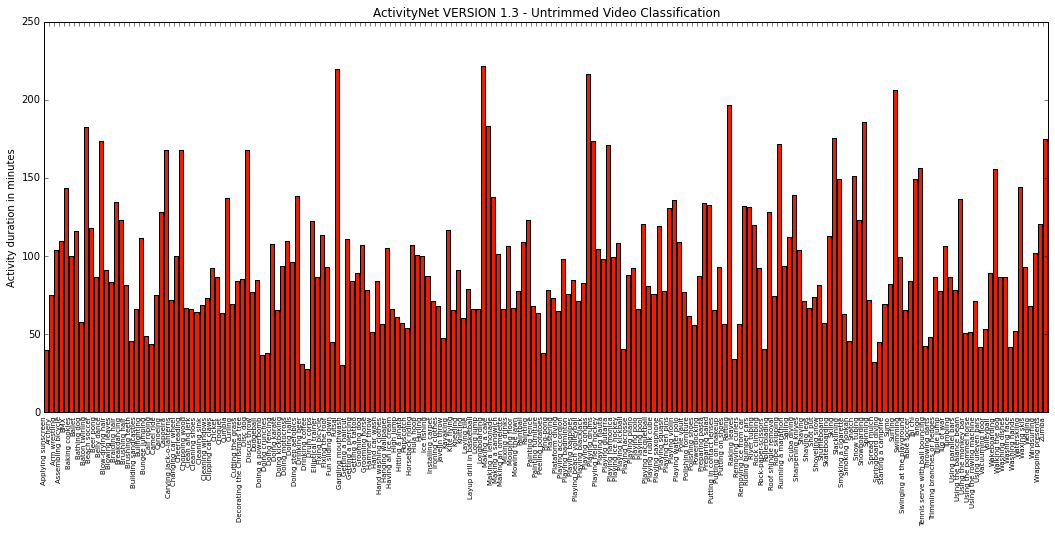
\includegraphics[width=1\linewidth]{img/methodology/dataset_stats}
\end{center}
\caption{Activity duration in minutes for each activity in the dataset}
\label{fig:dataset_stats}
\end{figure}

\section{Evaluation Metric}

In task like classification and detection, the research community and also the ActivityNet Challenge use the same metrics for evaluation to be able to compare results between publications. For the classification tasks, for each instance more than one prediction can be made, and for each prediction giving a the probability of success computed. With this multiple predictions for each instance some metric are computed. The simplest one is the \textit{Hit@k}, which gives you the proportion of the instance where the ground truth is on the \textit{top-k} predictions given. For the ActivityNet Challenge $k$ was set to 3.

In addition to this metric, for classifications tasks, it is mostly use the mean Average Precision (mAP) metric. It is computed as the mean of the average precision of all $M$ classes at the Dataset.

\begin{equation}
	mAP = \frac{1}{M} \sum_{m=1}^{M} AP(m)
\end{equation}

At the same time, the Average Precision for each class is computed as the average of the precision at position $n$, showed as $P(n)$. This precision is defined as the amount of elements in $k_m$ between positions 1 and $n$ in the ranked list divided by $n$.

\begin{equation}
	AP(m) = \frac{1}{k_m} \sum_{n=1}^{k_m} P(n)
\end{equation}

For the other task of the Challenge, the temporal localization or detection as the Challenge name it, the metric use to verify the results given is the Intersection Over Union (IoU). This metric compute a prediction as correct if the IoU of the prediction with the ground truth annotations is higher than a value $\alpha$. Then the mAP is computed. For the ActivityNet Challenge the $\alpha$ value used is 0.5.

For all the metrics computations of this section, it has been used the evaluation scripts given by the ActivityNet Challenge 2016 organization.

\section{Classification Task}

The first experiments made were related to the Recurrent Neural Network architecture, in order to obtain the best performance. The way to measure the performance, was computing the mAP for the classification task. The different architectures first tested were related to the deep of the network. On the first experiment, it was tested from a 3 layers LSTM with 1024 cells each layer, to a one single layer with 512 cells, going through a two layers network with 512 LSTM cells each one. All the architectures presented a batch normalization after the input entrance and dropout before and after the LSTM layers. Also all the experiments were done exclusively with the features extracted from the C3D network.

As is showed on Table~\ref{table:classification_by_architecture}, the network that achieved the best performance was achieved with the simplest one as was expected while training due to the fact that all the networks presented high learning capacity over our data.

\begin{table}[H]
\begin{center}
\begin{tabular}{|l|c|c|}
\hline
Architecture & mAP & Hit@3 \\
\hline\hline
3 x 1024-LSTM & 0.5635 & 0.7437 \\
2 x 512-LSTM & 0.5492 & 0.7364 \\
1 x 512-LSTM & \bf0.5938 & \bf0.7576 \\
\hline
\end{tabular}
\end{center}
\caption{Results for classification task comparing different deep architectures. All values with
         only video features on the validation dataset.}
\label{table:classification_by_architecture}
\end{table}

Once the best architecture was chosen in the sense of deepness, the network was trained comparing the input features used and also comparing the basic architecture with the one that feedback from the previous output. On the Table~\ref{table:classification_by_features} can be seen how the basic architecture and with only features from the video obtain the best results.

\begin{table}[H]
\begin{center}
\begin{tabular}{|l|c|c|}
\hline
Features used & mAP & Hit@3 \\
\hline\hline
Only video & \bf0.5938 & \bf0.7576 \\
Video w/ audio & 0.5755 & 0.7352 \\
Only video \& feedback & 0.5210 & 0.6982 \\
Video w/ audio \& feedback & 0.5652 & 0.7319 \\
\hline
\end{tabular}
\end{center}
\caption{Results for classification task with the model made by one 512-LSTM. Compare between
         features and feedback on the validation dataset.}
\label{table:classification_by_features}
\end{table}

%%%%%%
How I justify that with audio features the results are worst?
%%%%%%

The ActivityNet Dataset offers a 200 activities videos, but all this activities come from a taxonomy with hierarchically activities. The 200 activities which are annotated all the videos of the dataset and the proposed network predict are the leaf nodes of the taxonomy tree. On this structure there is 5 top level categories which all the videos belongs and describe more generally the activity happening on the video. These are: \textit{Eating and drinking activities}, \textit{Sports, Exercise and Recreation}, \textit{Household Activities}, \textit{Socializing, Relaxing and Leisure}, \textit{Personal Care}.

For all these top level activities, the mean average precision has been computed. To do so, all the predicted and ground truth activity labels have been changed by its top level activity and then for each of them computed the Average Precision. As can be seen on Table~\ref{table:top_level_classification_ap} and Figure~\ref{table:top_level_classification_ap} the \textit{Sports, Exercise and Recreation} have an average precision of $94\%$. This can be explained with the fact that all the features extracted from the videos come from a network which weights were trained to work with a dataset of videos, the Sports1M\cite{KarpathyCVPR14}.

\begin{table}[H]
\begin{center}
\begin{tabular}{|r|c|}
\hline
\textbf{Global Activities} & \textbf{AP} \\
\hline\hline
Eating and drinking Activities & 0.56942 \\
Sports, Exercise, and Recreation & 0.93662 \\
Household Activities & 0.74177 \\
Socializing, Relaxing, and Leisure & 0.76494 \\
Personal Care & 0.59931 \\
\hline\hline
\textbf{Global} (mAP) & 0.72241 \\
\textbf{Global} (Hit@3) & 0.92703 \\
\hline
\end{tabular}
\end{center}
\caption{Mean Average Precision computed for the top level activities of the ActivityNet Dataset. The results are computed over the validation dataset.}
\label{table:top_level_classification_ap}
\end{table}

\begin{figure}[H]
\begin{center}
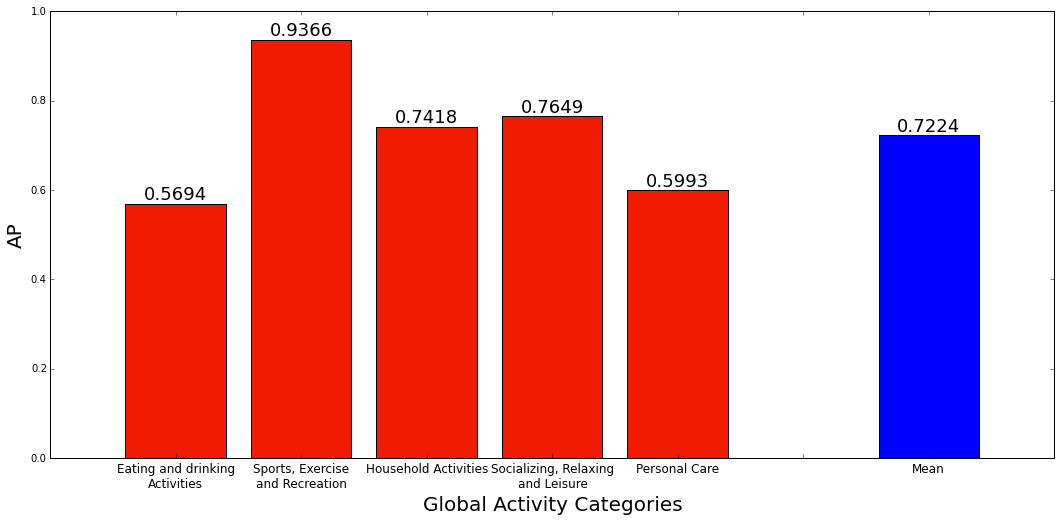
\includegraphics[width=1\linewidth]{img/results/top_activities_classification_ap}
\end{center}
\caption{Representation of the results over the top-level activities}
\label{fig:top_level_classification_ap}
\end{figure}



\begin{figure}[H]
\begin{center}
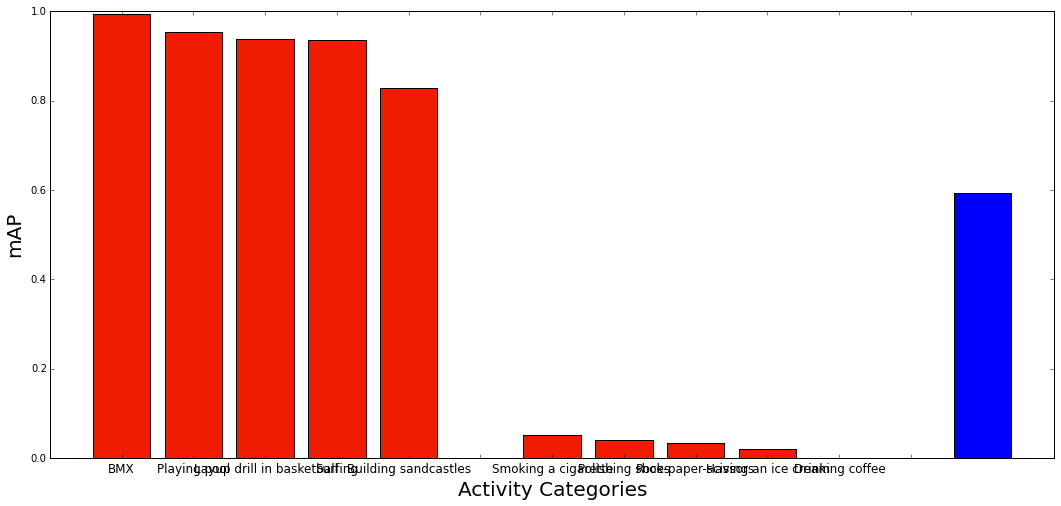
\includegraphics[width=1\linewidth]{img/results/high_low_map_classification}
\end{center}
\caption{Sample of activities with the highest and lowest mAP for the classification task}
\label{fig:map_by_activity_classification}
\end{figure}

\begin{figure}[H]
\begin{center}
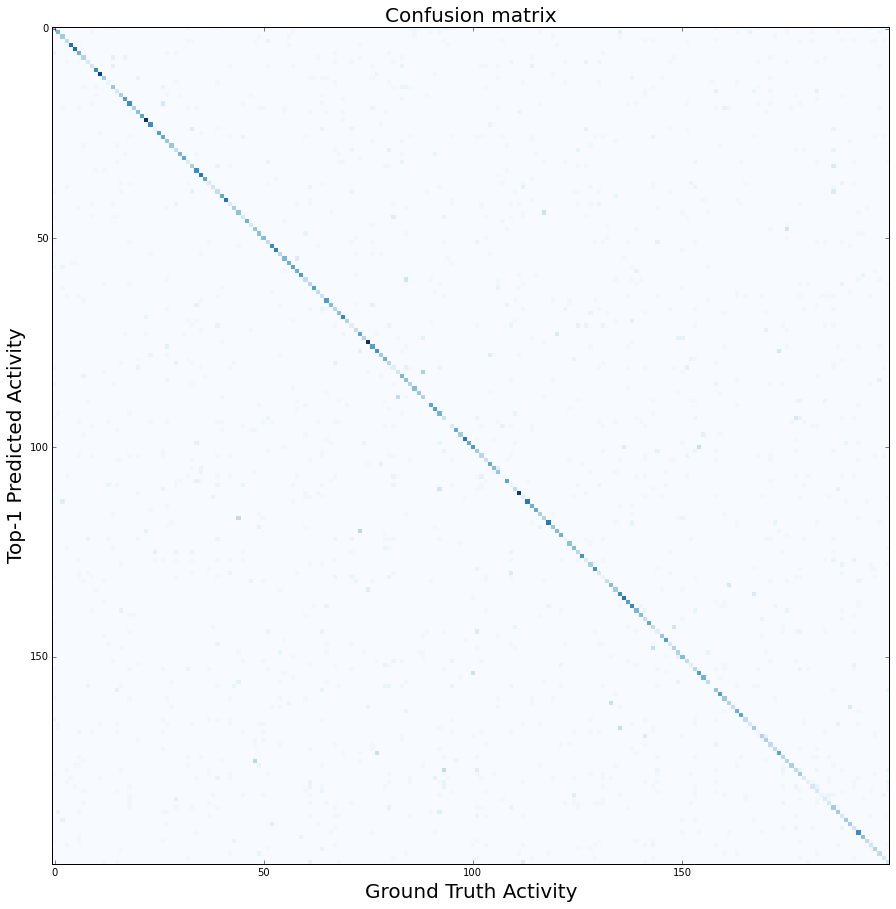
\includegraphics[width=1\linewidth]{img/results/confussion_matrix}
\end{center}
\caption{Confusion matrix of the top-1 activity predicted with the ground truth}
\label{fig:confussion_matrix}
\end{figure}

%%%%%%%%%%%
You think the confusion matrix is good idea to putting on the memory. Annex!!!!
%%%%%%%%%%%

At the time of submitting the predictions made with the best model for the testing dataset the mAP obtained was of $0.58741$ and the Hi@3 of $0.75548$.

\section{Detection Task}

As the main goal of this project is to obtain a good network to temporally localize activities on videos, it has been compared the results on the detection task of the ActivityNet Challenge for the two architectures proposed. For the basic architecture the network was feed up with video features from the C3D network, while on the feedback architecture, the audio features were concatenated at the input as in classification task improve the results (check Table~\ref{table:classification_by_features}).

%%%%%%%%
How I justify the feedback architecture does not give best results than the basic one?
%%%%%%%%

\begin{table}[H]
\begin{center}
\begin{tabular}{|l|c|}
\hline
Architecture & mAP \\
\hline\hline
Basic Architecture & \bf0.22513 \\
Feedback Architecture & 0.20676 \\
\hline
\end{tabular}
\end{center}
\caption{Best results obtain for the temporal activity localization task in the two architectures}
\label{table:detection_architecture_comparison}
\end{table}

As shows the Table~\ref{table:detection_architecture_comparison} the basic architecture get a slightly better results. The computation of the mean average precision was done doing the same post-processing to the predicted output of the network proposed on this project.

As it was explained on Section~\ref{section:post_processing}, a post-processing was done to the output to achieve a smoother and better temporal prediction of the activities. During this project there were performed some experiments to maximize the prediction precision for different values of $\gamma$ as the activity probability threshold and $k$ as smoothing factor for the mean filter. For different combinations of these variables it was performed the Table~\ref{table:detection_postprocessing_comparison}.

\begin{table}[H]
\begin{center}
\begin{tabular}{|l|c|c|c|}
\hline
$\gamma$ & $k=0$ & $k=5$ & $k=10$ \\
\hline
0.2 & 0.20732 & \bf0.22513 & 0.22136 \\
0.3 & 0.19854 & 0.22077 & 0.22100 \\
0.5 & 0.19035 & 0.21937 & 0.21302 \\
\hline
\end{tabular}
\end{center}
\caption{mAP with an IOU threshold of $0.5$ over validation dataset. Here there is a comparison
between values of $k$ and $\gamma$ on post processing.}
\label{table:detection_postprocessing_comparison}
\end{table}

As can be seen, the best performance was achieved with an activity threshold $\gamma=0.2$ and smoothing filter of $k=5$. The effect of the both of the operations performed after the prediction can be seen on Figures~\ref{fig:smoothing_effect} and~\ref{fig:activty_threshold_effect}. On both figures it is displayed temporally the location of the activity at the ground truth of the video and also the prediction done with the proposed network before and after of each of the post-processing.

\begin{figure}[H]
\begin{center}
%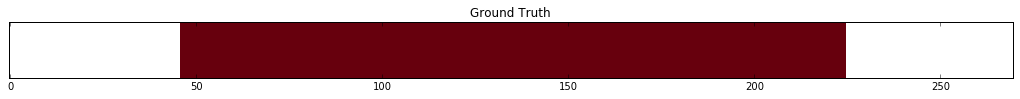
\includegraphics[width=1\linewidth]{img/results/smoothing_effect_1}
%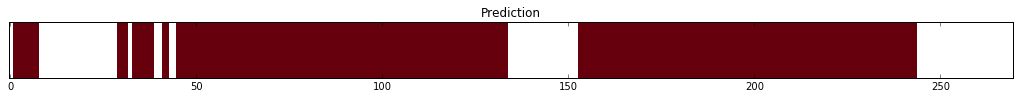
\includegraphics[width=1\linewidth]{img/results/smoothing_effect_2}
%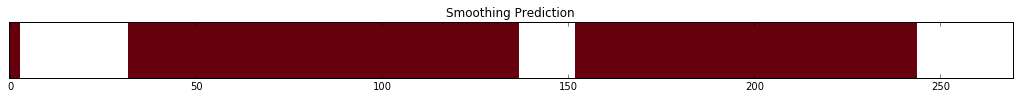
\includegraphics[width=1\linewidth]{img/results/smoothing_effect_3}
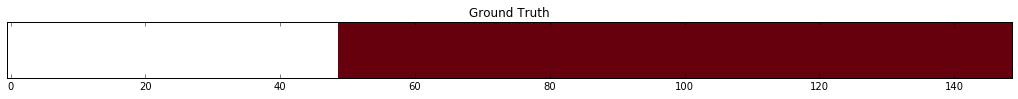
\includegraphics[width=1\linewidth]{img/results/smoothing_effect_4}
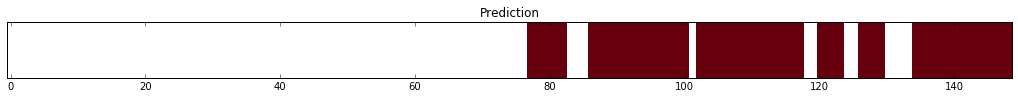
\includegraphics[width=1\linewidth]{img/results/smoothing_effect_5}
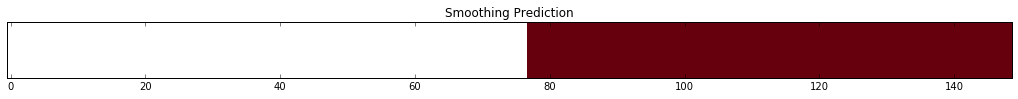
\includegraphics[width=1\linewidth]{img/results/smoothing_effect_6}
\end{center}
\caption{Effect of the mean filter with $k=5$ achieving a smoother activity prediction.}
\label{fig:smoothing_effect}
\end{figure}

\begin{figure}[H]
\begin{center}
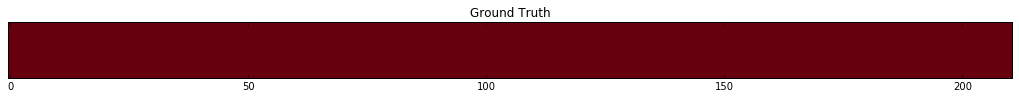
\includegraphics[width=1\linewidth]{img/results/activity_threshold_effect_1}
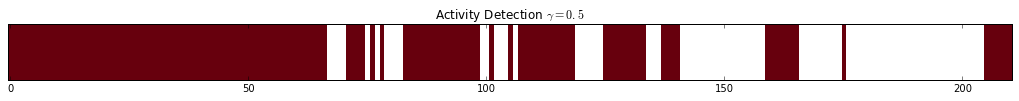
\includegraphics[width=1\linewidth]{img/results/activity_threshold_effect_2}
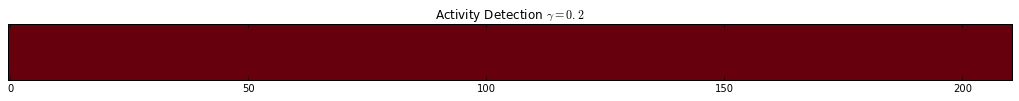
\includegraphics[width=1\linewidth]{img/results/activity_threshold_effect_3}
\end{center}
\caption{}
\label{fig:activty_threshold_effect}
\end{figure}

As it has been done for the classification task, the Average Precision has been computed for the top level activities of the ActivityNet Dataset taxonomy. As can be seen on Table~\ref{table:top_level_detection_ap} and Figure~\ref{fig:top_level_detection_ap} all the top level activities present a similar precision in activity temporal localization except from the category \textit{Personal Care} which does not achieve the half of precision of the rest of top level categories. Also remark that the top level category with highest precision is \textit{Sports, Exercise and Recreation} as happens on the classification task.

\begin{table}[H]
\begin{center}
\begin{tabular}{|r|c|}
\hline
\textbf{Global Activities} & \textbf{AP} \\
\hline\hline
Eating and drinking Activities & 0.25582 \\
Sports, Exercise, and Recreation & 0.30023 \\
Household Activities & 0.26252 \\
Socializing, Relaxing, and Leisure & 0.26060 \\
Personal Care & 0.11234 \\
\hline\hline
\textbf{Global} (mAP) & 0.23830 \\
\hline
\end{tabular}
\end{center}
\caption{Average Precision of activity localization computed for the top level activities of the ActivityNet Dataset. The results are computed over the validation dataset and with a IoU threshold of 0.5.}
\label{table:top_level_detection_ap}
\end{table}

\begin{figure}[H]
\begin{center}
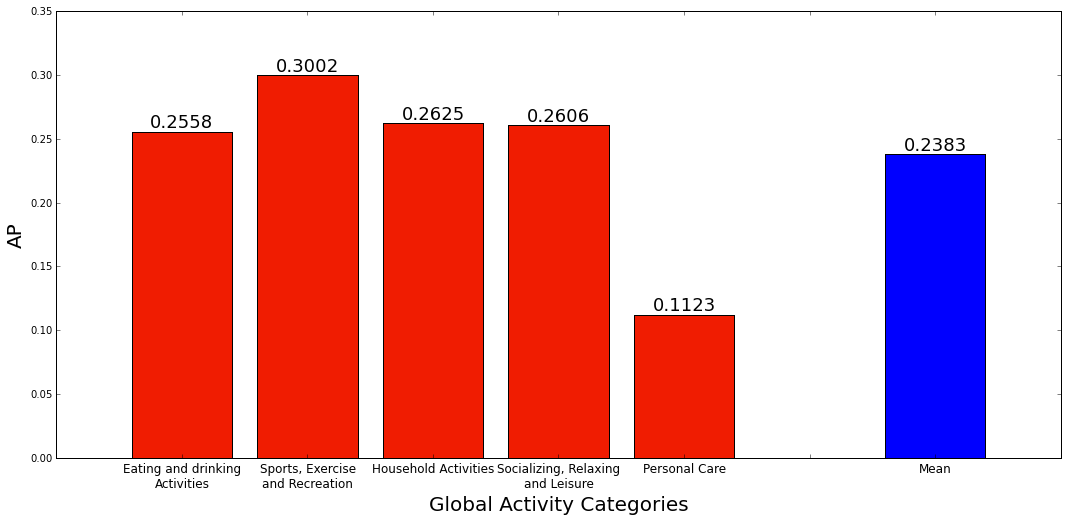
\includegraphics[width=1\linewidth]{img/results/top_activities_detection_ap}
\end{center}
\caption{Representation of the results over the top-level activities}
\label{fig:top_level_detection_ap}
\end{figure}

\begin{figure}[H]
\begin{center}
%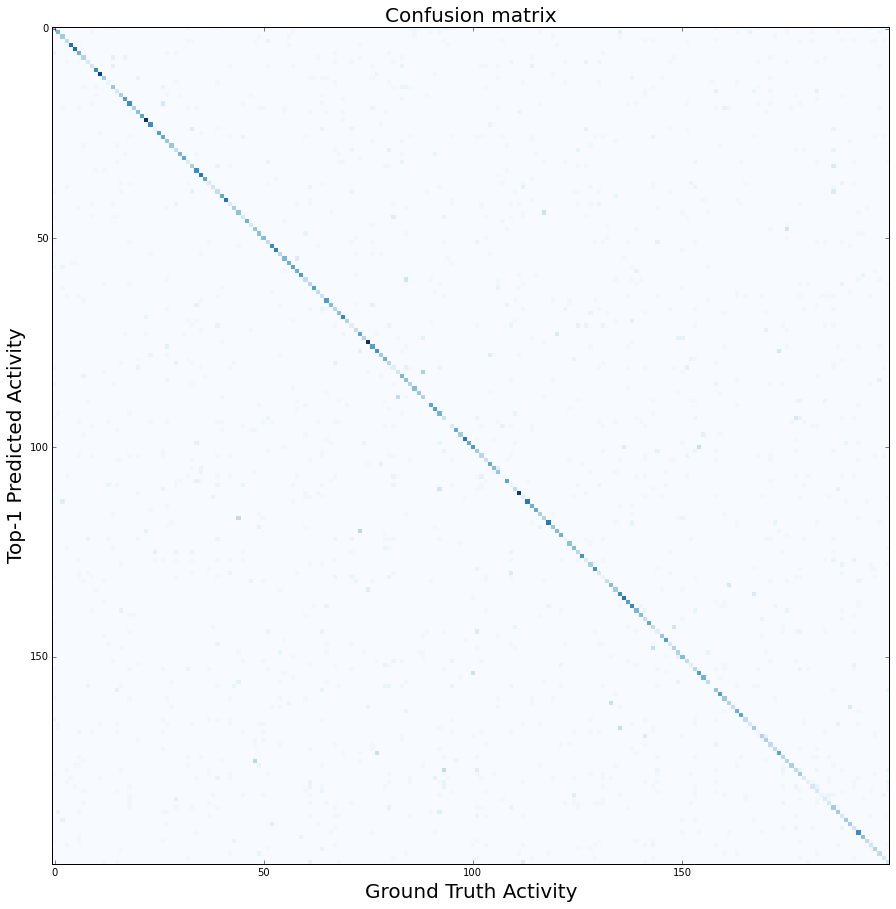
\includegraphics[width=1\linewidth]{img/results/confussion_matrix}
\end{center}
\caption{Activities with higher and lower mAP for the detection task}
\label{fig:map_by_activity_detection}
\end{figure}

%%%%%%%%
I don't know if the previous figure actually putting it
On the other hand I will put a figure plotting the mAP against the IoU asked between 0.1 and 0.5
%%%%%%%%

Plot with multiple IOU and mAP...

\section{Results Visualization}

Here attach some figures about the predictions made by our model.
Spend a whole page with examples of temporal predictions.

Doubt: put the figures as the ground truth and classes predicted in a scale of colors,
or plot only the part of the ground truth that has an activity and also the prediction where the activity is placed as at is computed in the post-processing to compare?


\chapter{Conclusions and Future Work}

To talk about on the conclusion:
\begin{itemize}
	\item Bad audio at the video and that's why the audio does not improve
    \item The C3D network was pre-trained for the Sports1M dataset so that's why the best score were to the sports categories.
    \item Why the simplest architecture gives better results (only be a little) than the feedback architecture
    \item Same results that other participant on the Challenge but using a more simplest network.
    \item good results taking into account that it has been all done from scratch.
\end{itemize}


As future work:
\begin{itemize}
    \item Use optical flow as input as used in paper \cite{simonyan2014two}\cite{Ng_2015_CVPR}\cite{Yao_2015_ICCV}
    \item Extract features of Conv layers rather than the first fc layer
    \item Improve with this hierarchy of action/background + classification (inspired by \cite{shoutemporal})
    \item Pre-traine networks to predict the next frame
    \item Train on 3D volumes (tubelets) directly
    \item Thumos challenge? If not try working with Thumos dataset\cite{THUMOS15}
    \item keep going the research line on the Image Processing group

\end{itemize}


\appendix
\chapter{Results Figures}

\begin{figure}[H]
\begin{center}
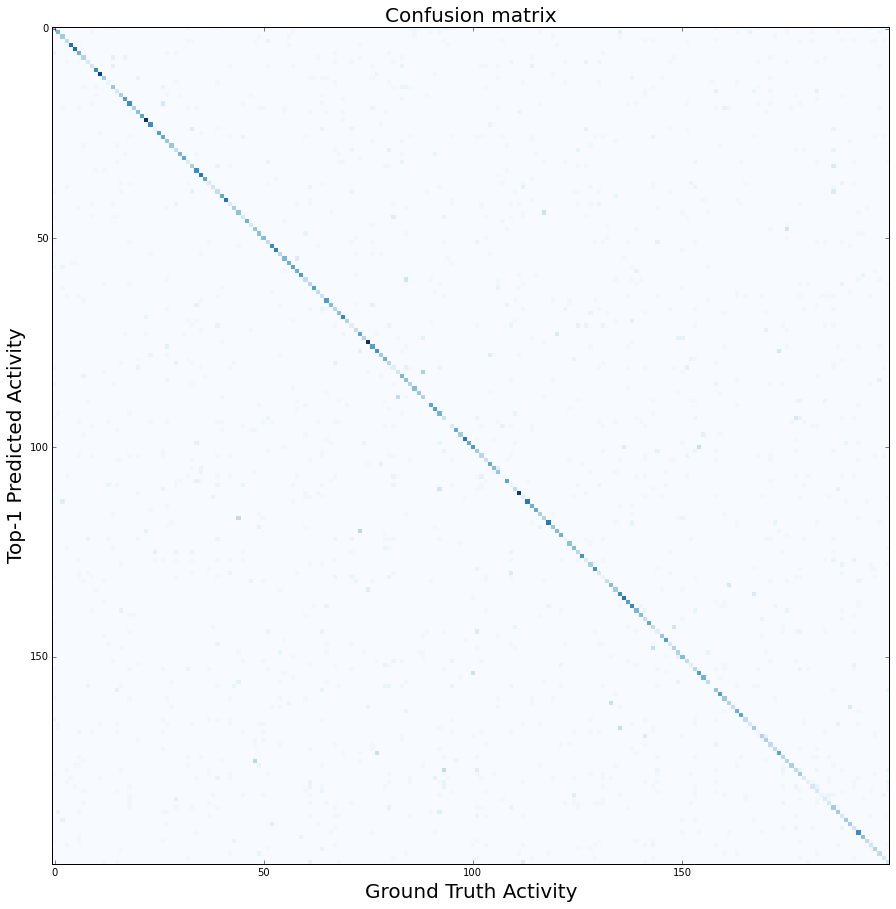
\includegraphics[width=1\linewidth]{img/results/confussion_matrix}
\end{center}
\caption{Confusion matrix of the top-1 activity predicted with the ground truth}
\label{fig:confussion_matrix}
\end{figure}


\begin{figure}[H]
\centering
\begin{subfigure}[b]{.4\textwidth}
  \texttt{Video ID: c-zbA4zixfE \\
  Activity: Throwing darts \\
  \\
  Prediction: \\
  0.7325	Throwing darts \\
  0.1364	Baking cookies \\
  0.0254	Playing blackjack \\}
\end{subfigure}%
\begin{subfigure}[b]{.6\textwidth}
  \centering
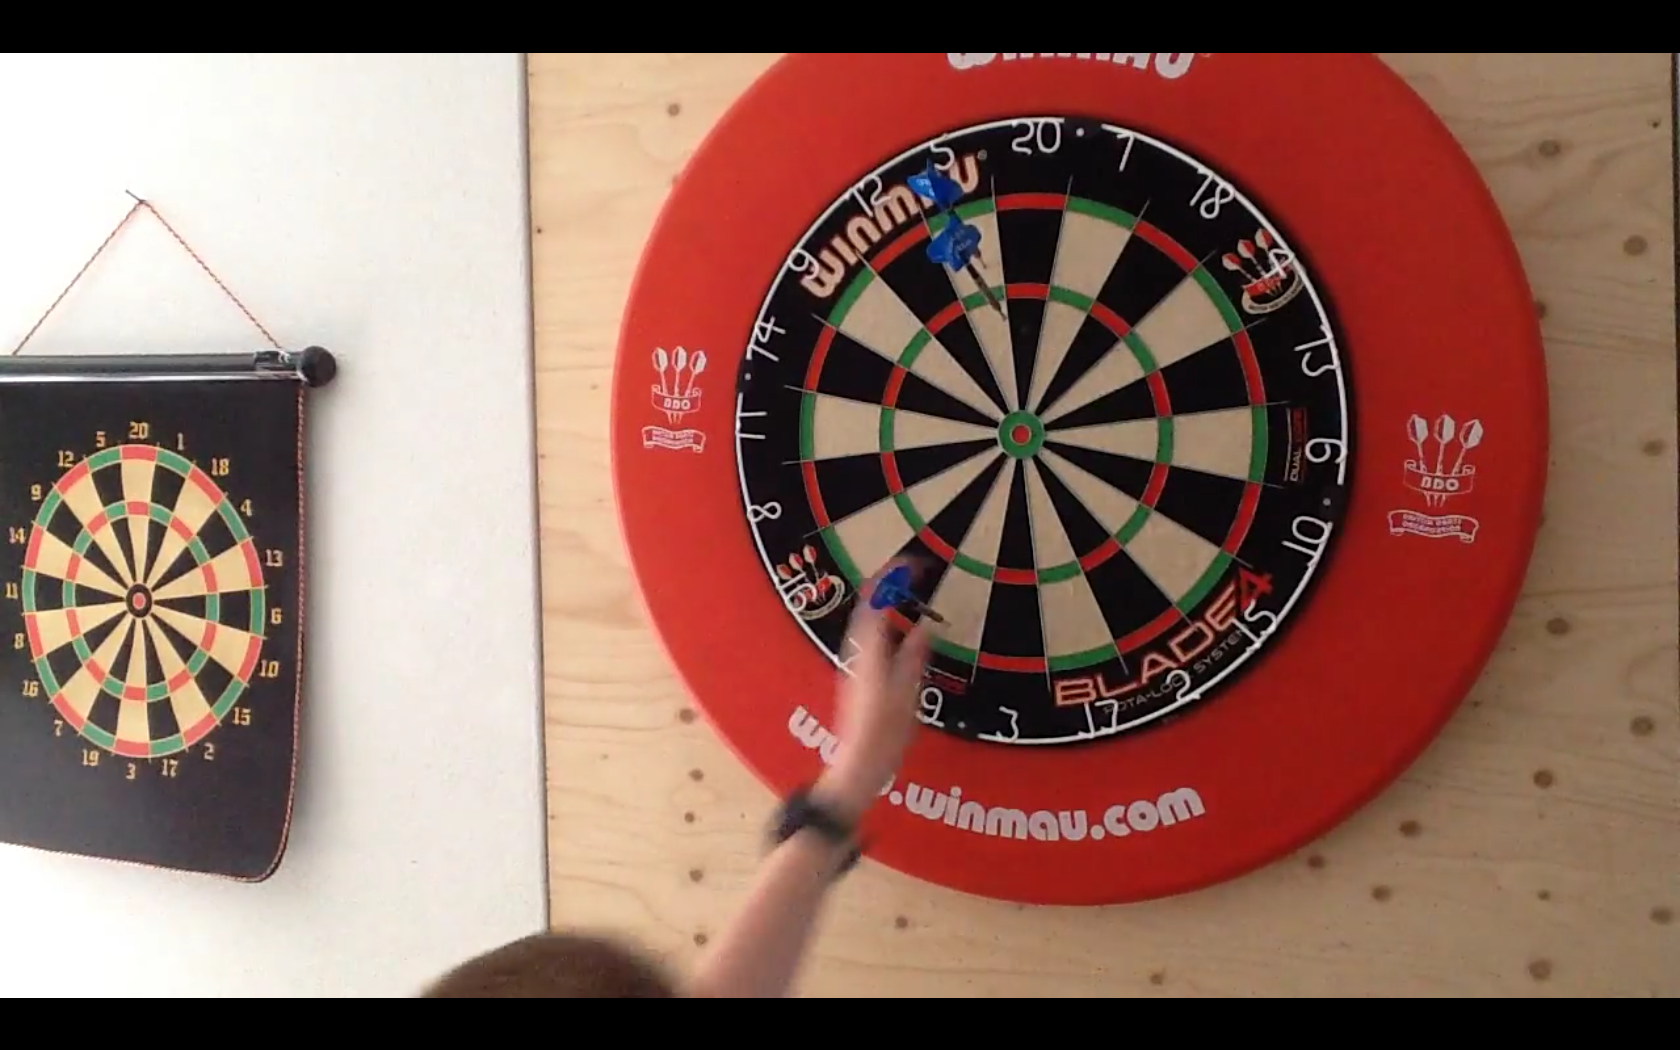
\includegraphics[width=0.95\linewidth]{img/results/activity_classification/results_visualization_classification_5}
\end{subfigure}

\begin{subfigure}[b]{.4\textwidth}
  \texttt{Video ID: p8MvTi8hJdE \\
    Activity: Snowboarding \\
    \\
    Prediction: \\
    0.5043	Skiing \\
    0.2683	Snowboarding \\
    0.1637	Snow tubing \\}
\end{subfigure}%
\begin{subfigure}[b]{.6\textwidth}
  \centering
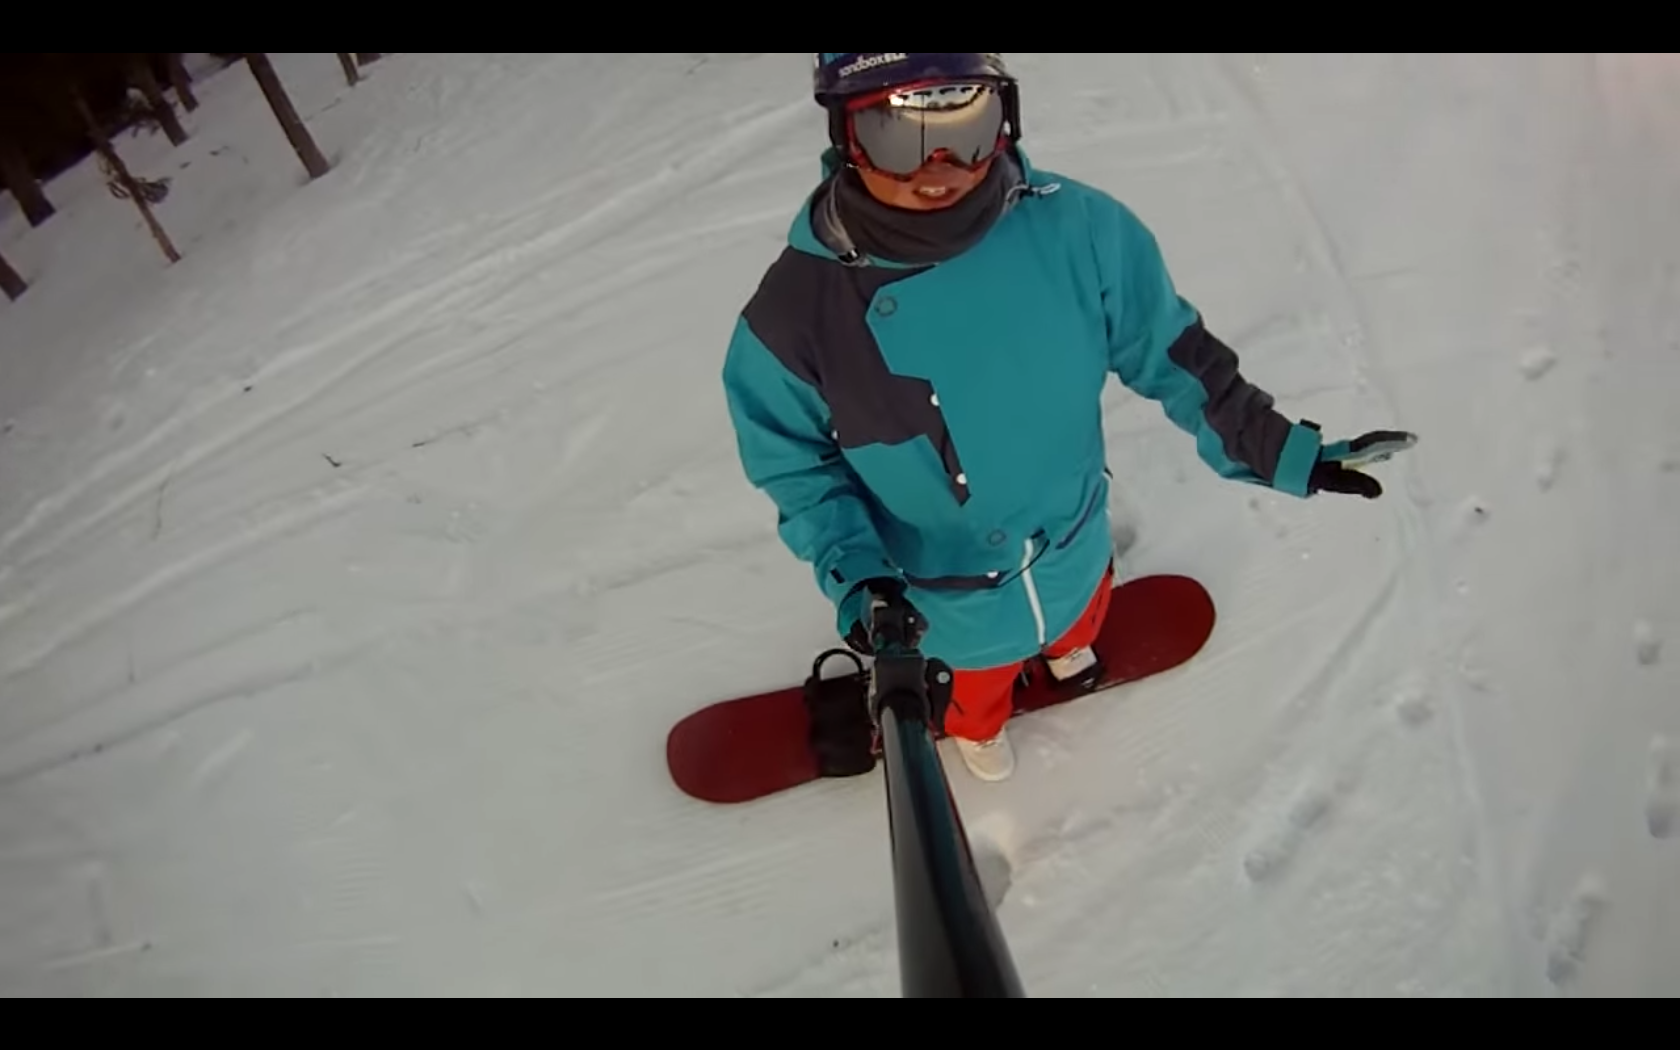
\includegraphics[width=0.95\linewidth]{img/results/activity_classification/results_visualization_classification_6}
\end{subfigure}

\begin{subfigure}[b]{.4\textwidth}
  \texttt{Video ID: ATk8OkvNHHQ \\
    Activity: BMX \\
    \\
    Prediction: \\
    0.9099	BMX \\
    0.0413	Doing motocross \\
    0.0103	Paintball \\}
\end{subfigure}%
\begin{subfigure}[b]{.6\textwidth}
  \centering
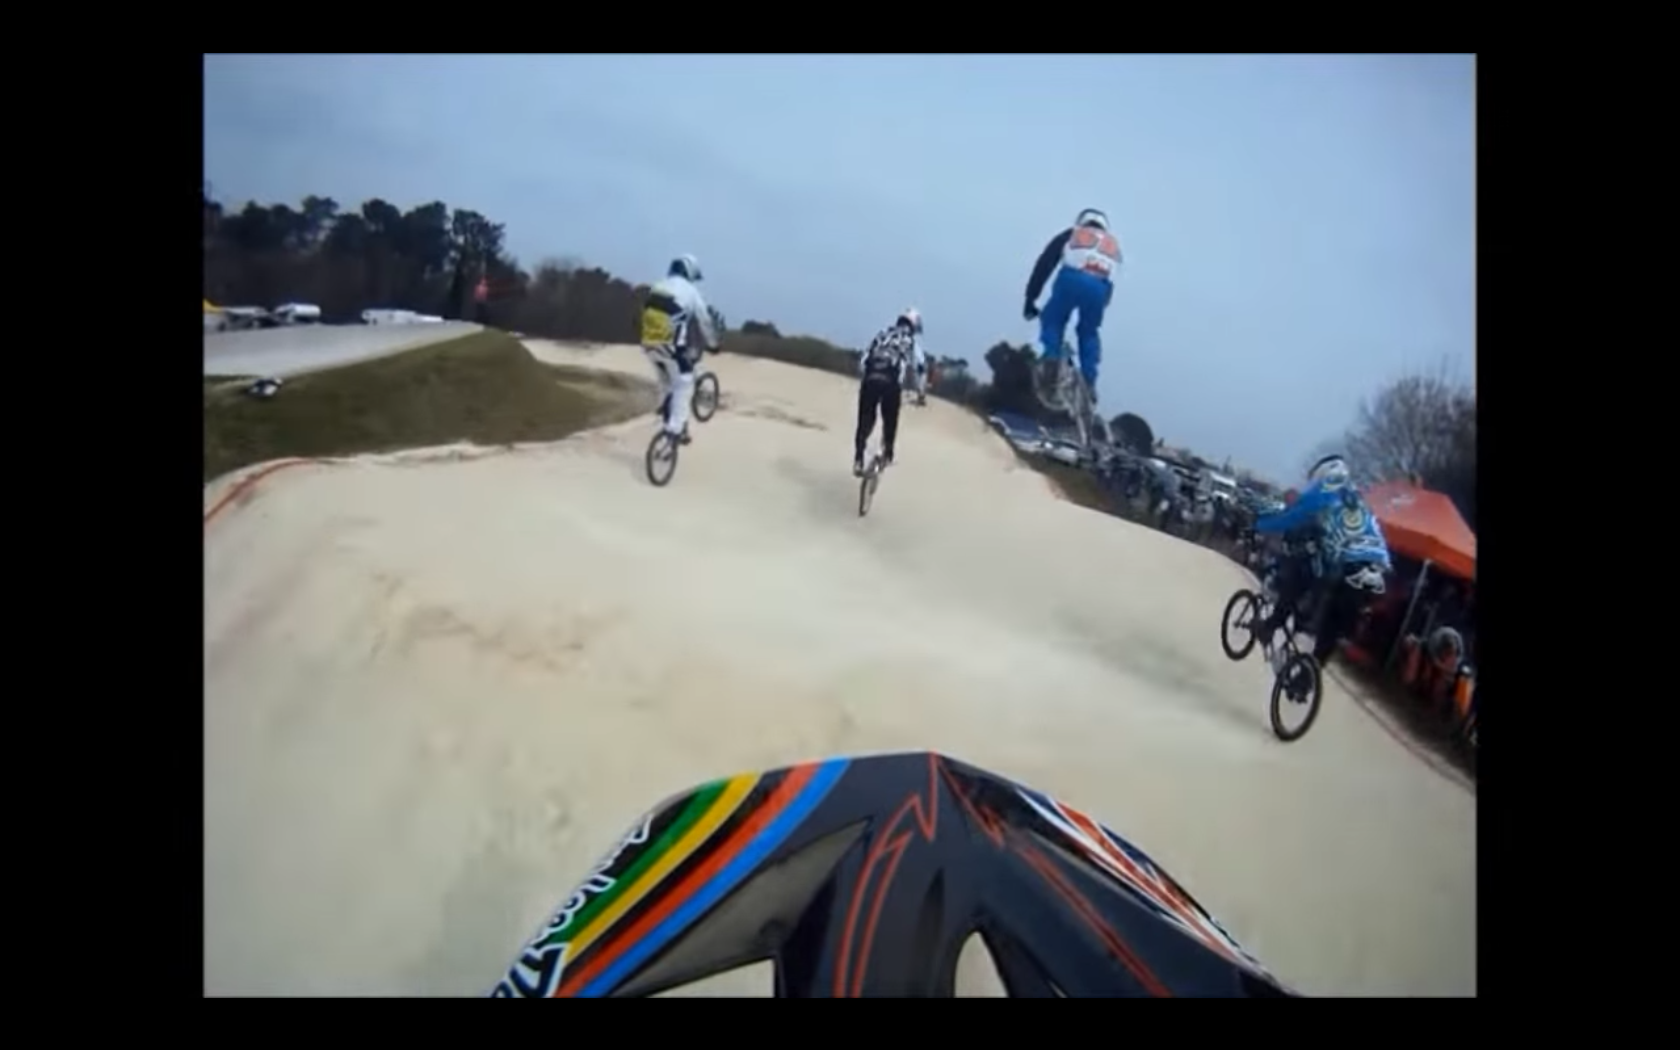
\includegraphics[width=0.95\linewidth]{img/results/activity_classification/results_visualization_classification_7}
\end{subfigure}

\begin{subfigure}[b]{.4\textwidth}
  \texttt{Video ID: -uR5-jYe0Ag \\
  Activity: Putting on makeup \\
  \\
  Prediction: \\
  0.1035	Smoking a cigarette \\
  0.1002	Getting a haircut \\
  0.0941	Putting on makeup \\}
\end{subfigure}%
\begin{subfigure}[b]{.6\textwidth}
  \centering
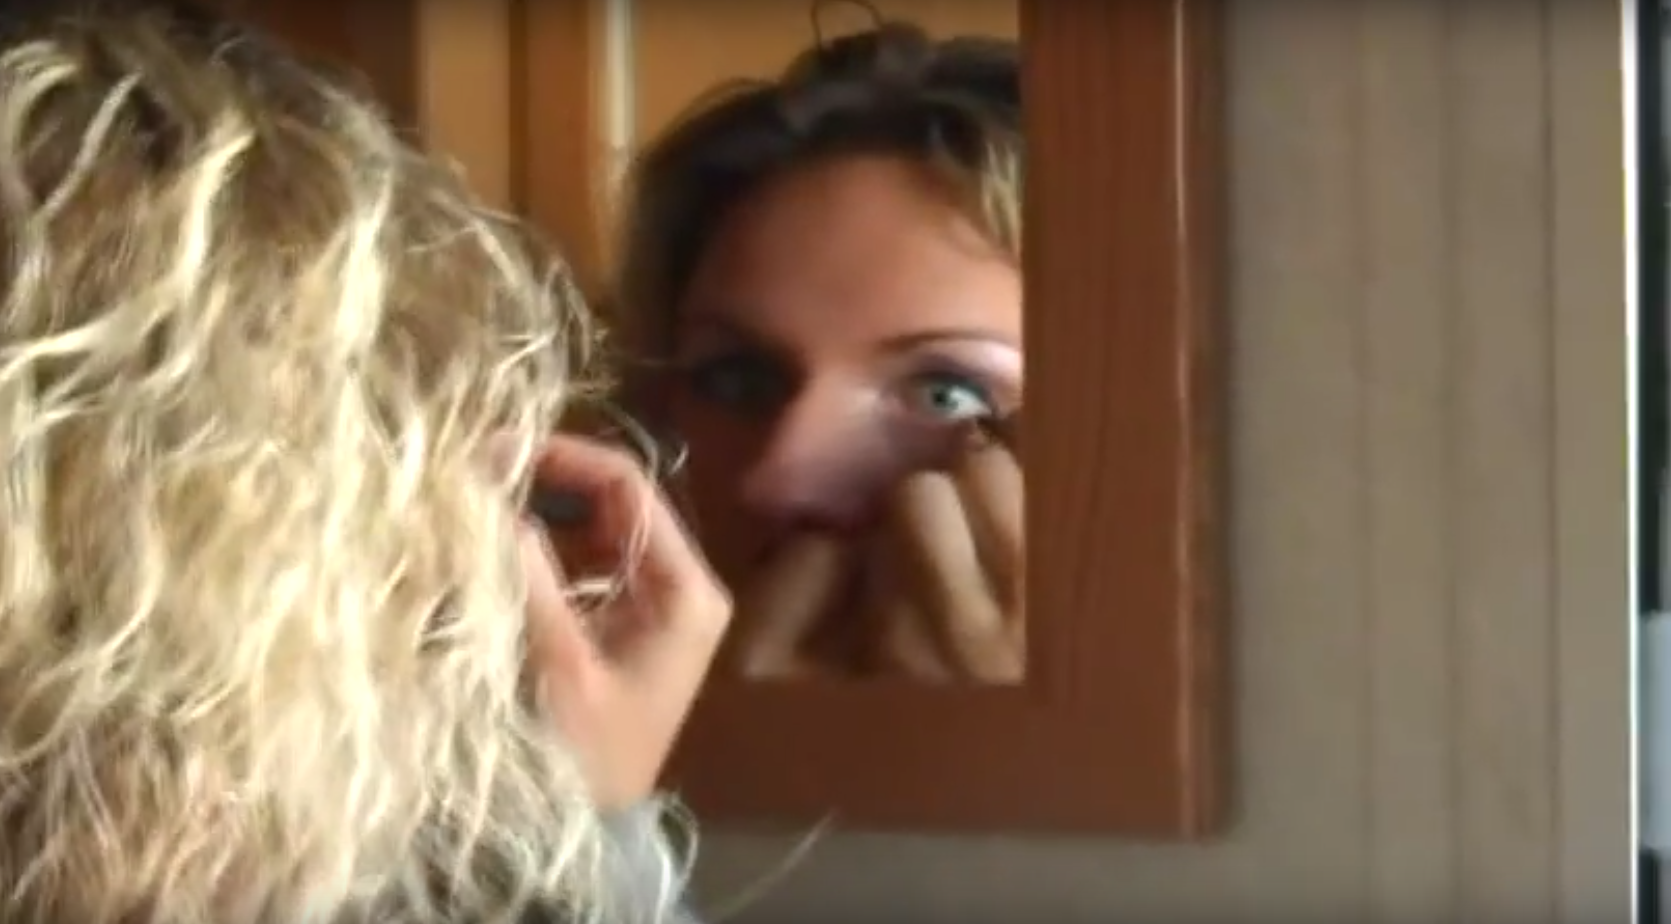
\includegraphics[width=0.95\linewidth]{img/results/activity_classification/results_visualization_classification_8}
\end{subfigure}

\caption{Results for the classification task}
\label{fig:results_visualization_classification_annex_1}
\end{figure}

\begin{figure}[H]
\centering
\begin{subfigure}[b]{.4\textwidth}
  \texttt{Video ID: vc820BteGzY \\
    Activity: Making a cake \\
    \\
    Prediction: \\
    0.3165	Making a lemonade \\
    0.1073	Putting on makeup \\
    0.0768	Making a cake \\}
\end{subfigure}%
\begin{subfigure}[b]{.6\textwidth}
  \centering
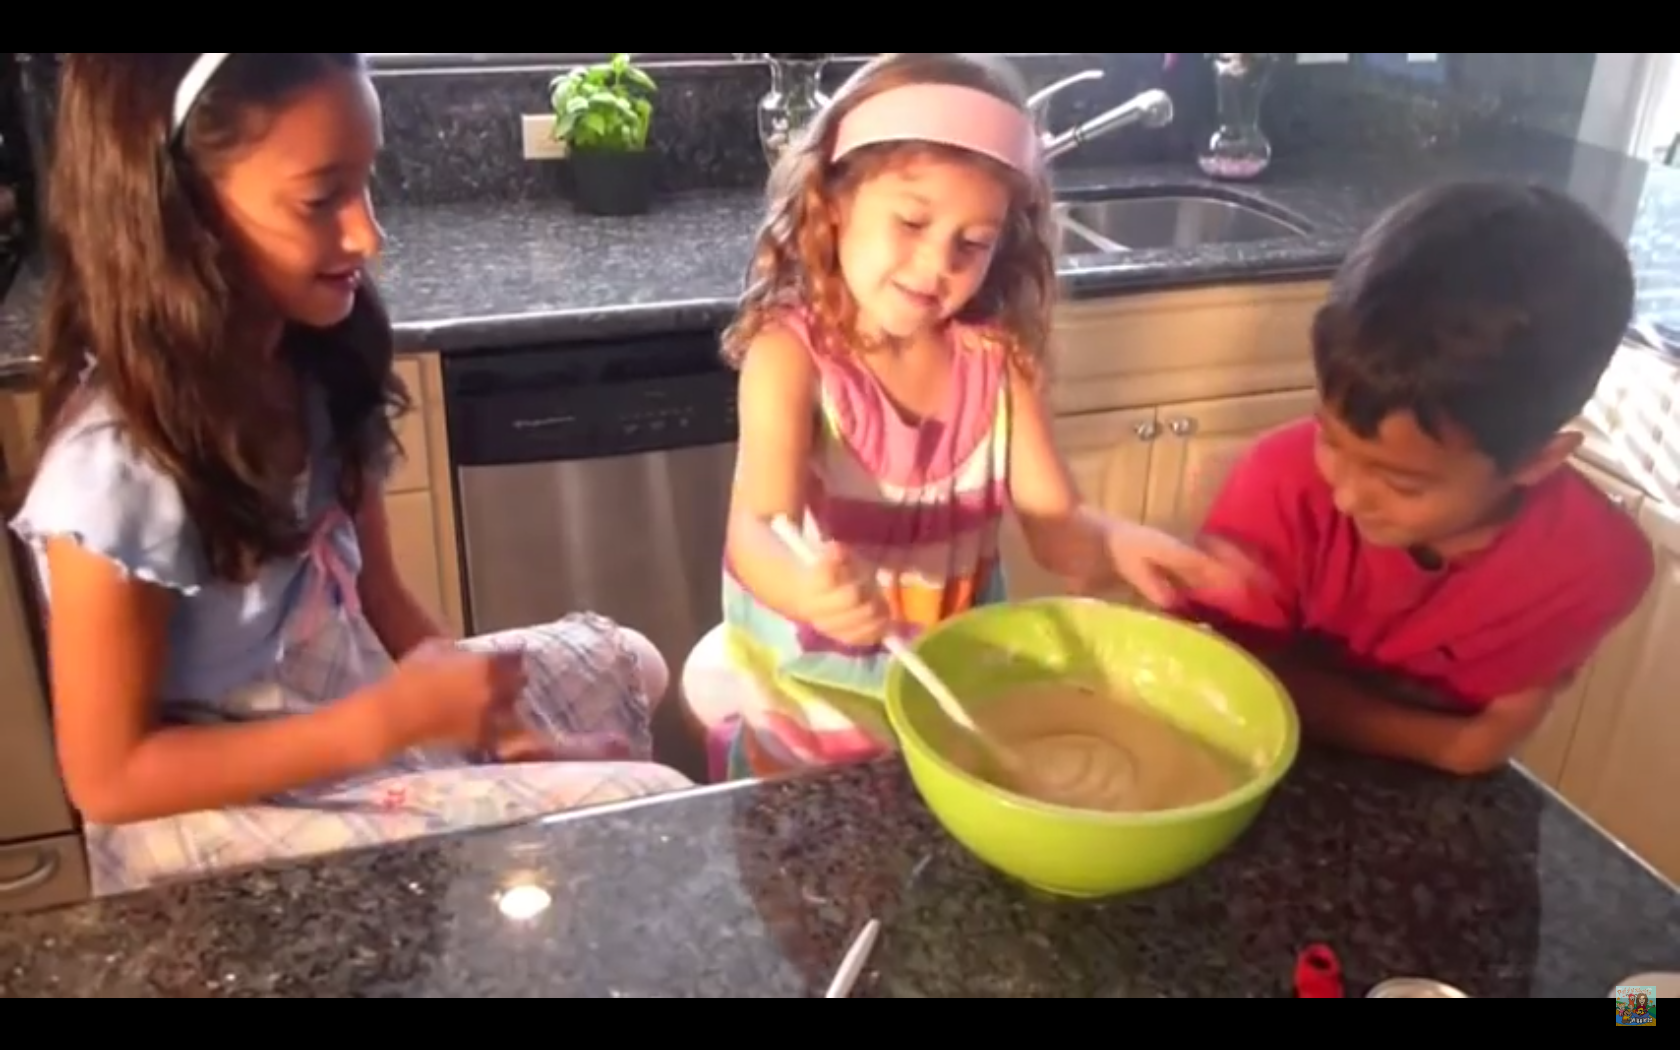
\includegraphics[width=0.95\linewidth]{img/results/activity_classification/results_visualization_classification_9}
\end{subfigure}

\begin{subfigure}[b]{.4\textwidth}
  \texttt{Video ID: tBNOJJx4Z9k \\
    Activity: Hand washing clothes \\
    \\
    Prediction: \\
    0.4742	Cleaning sink \\
    0.0728	Washing hands \\
    0.0497	Baking cookies \\}
\end{subfigure}%
\begin{subfigure}[b]{.6\textwidth}
  \centering
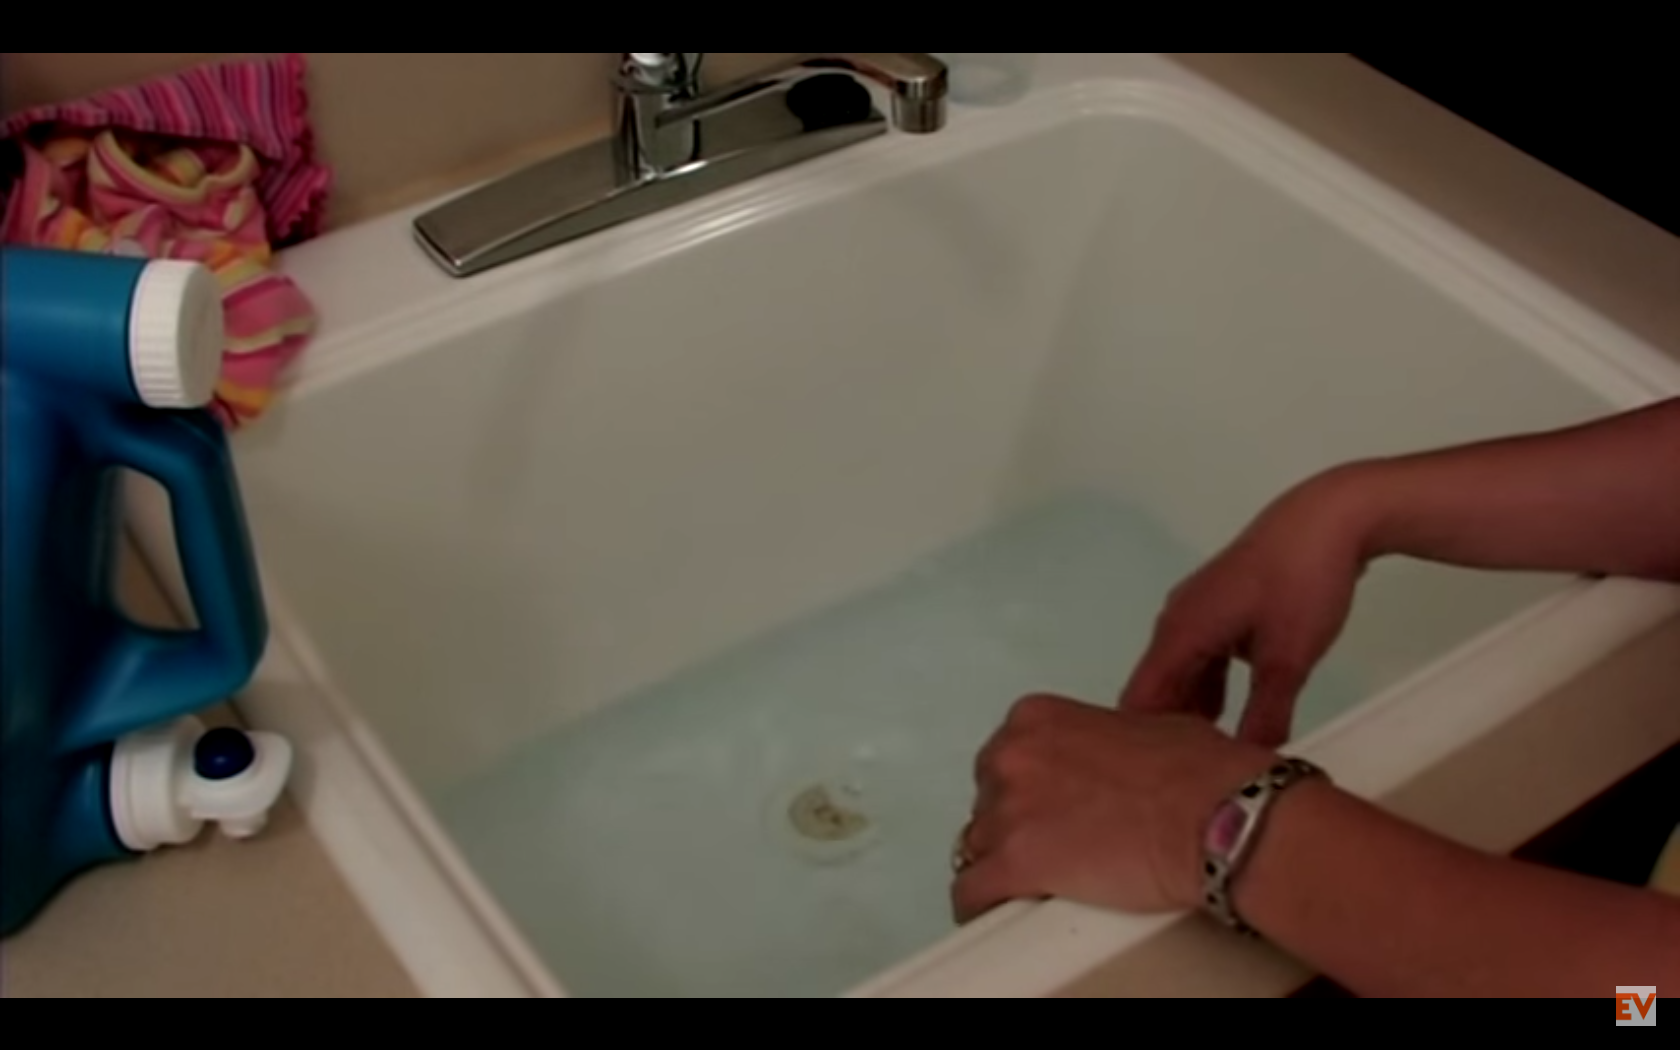
\includegraphics[width=0.95\linewidth]{img/results/activity_classification/results_visualization_classification_10}
\end{subfigure}

\begin{subfigure}[b]{.4\textwidth}
  \texttt{}
\end{subfigure}%
\begin{subfigure}[b]{.6\textwidth}
  \centering
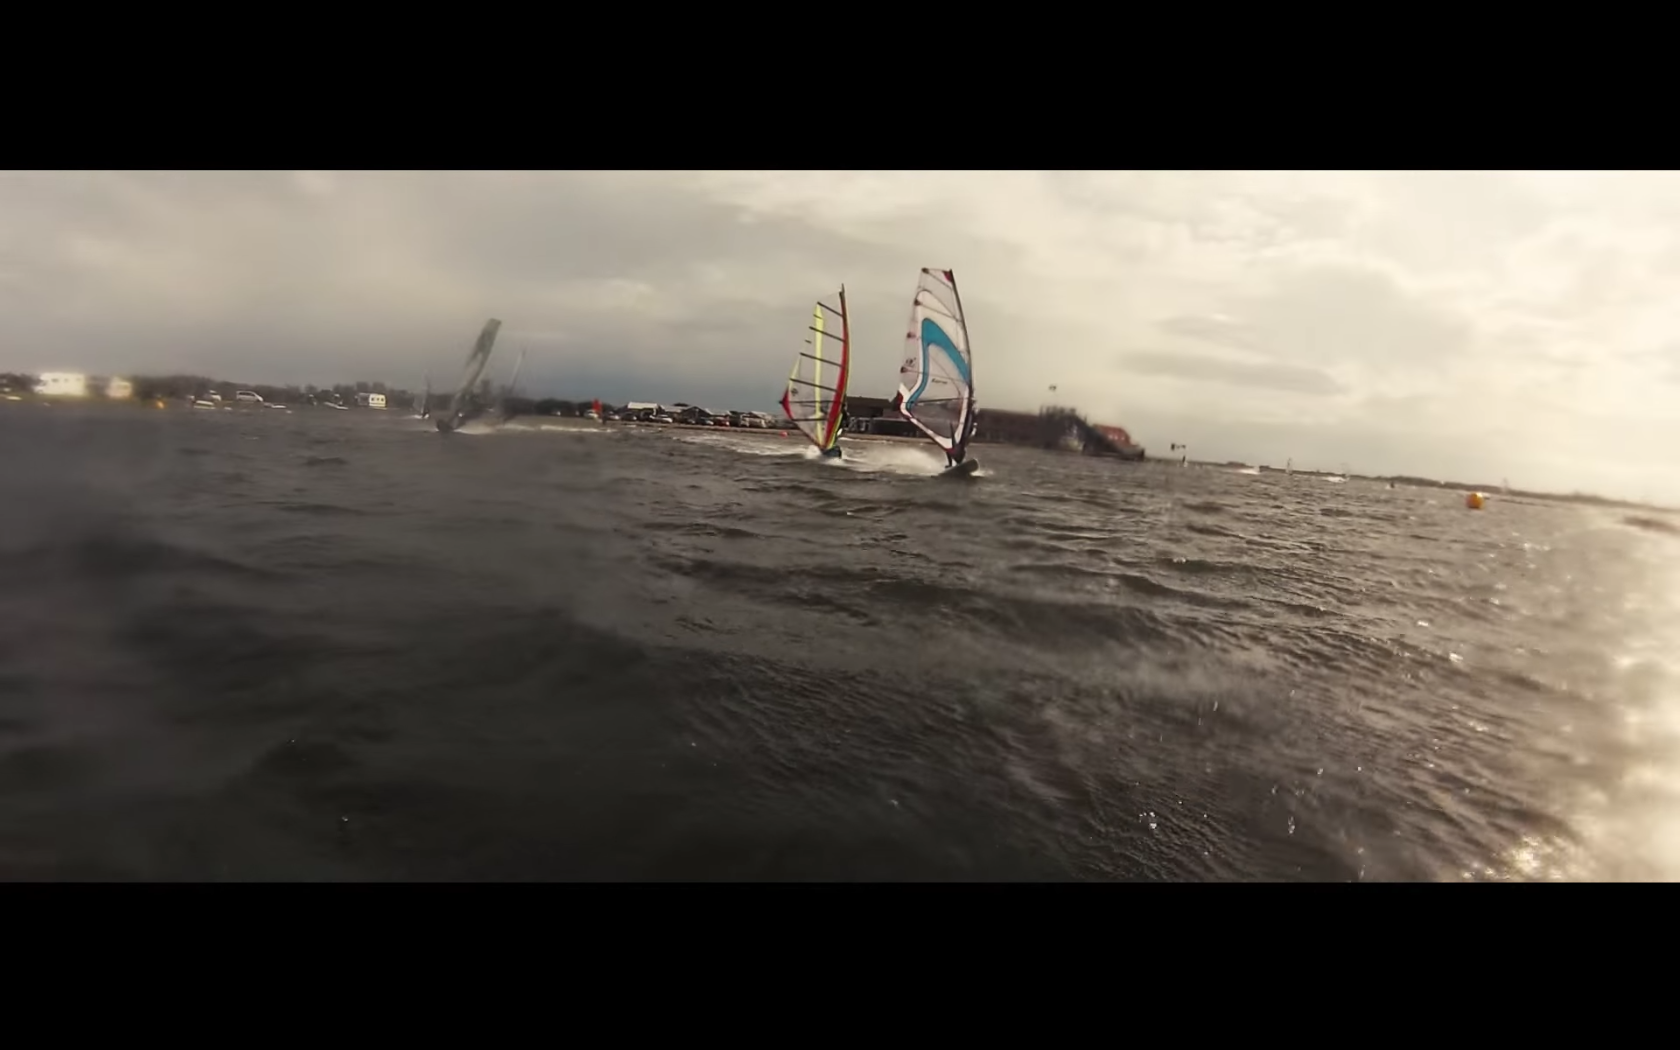
\includegraphics[width=0.95\linewidth]{img/results/activity_classification/results_visualization_classification_11}
\end{subfigure}

\begin{subfigure}[b]{.4\textwidth}
  \texttt{}
\end{subfigure}%
\begin{subfigure}[b]{.6\textwidth}
  \centering
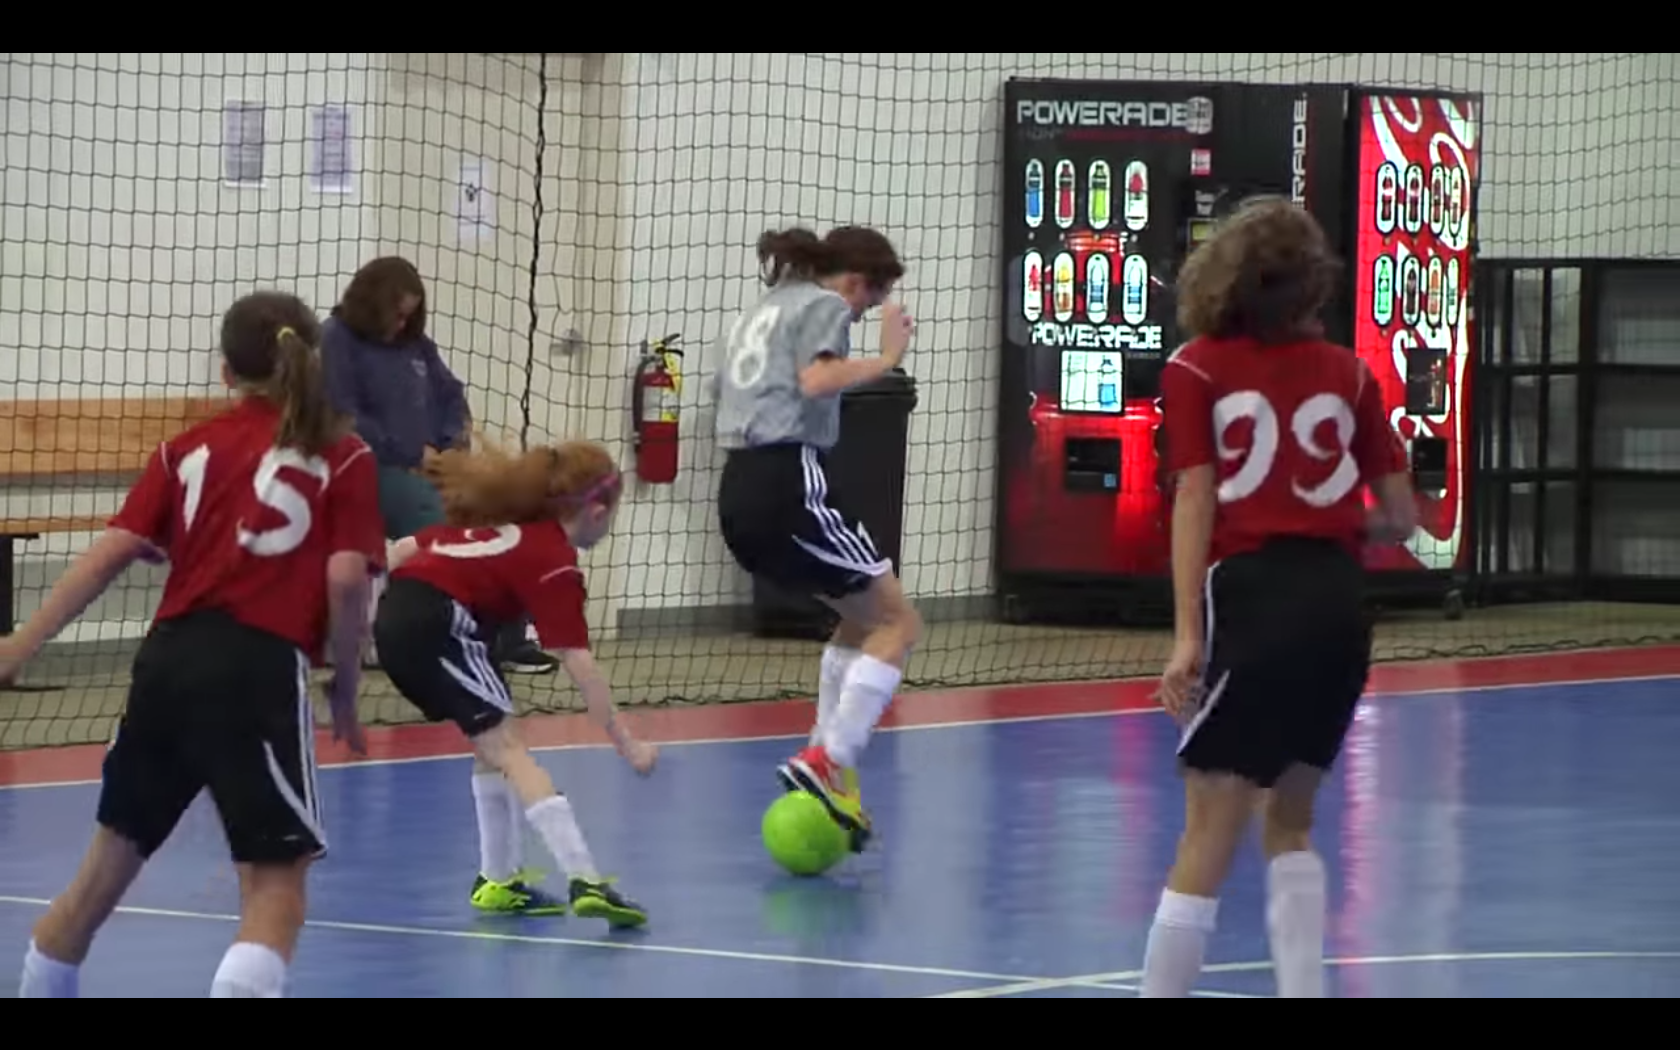
\includegraphics[width=0.95\linewidth]{img/results/activity_classification/results_visualization_classification_12}
\end{subfigure}

\caption{Results for the classification task}
\label{fig:results_visualization_classification_annex_2}
\end{figure}


\begin{figure}[H]
\begin{center}
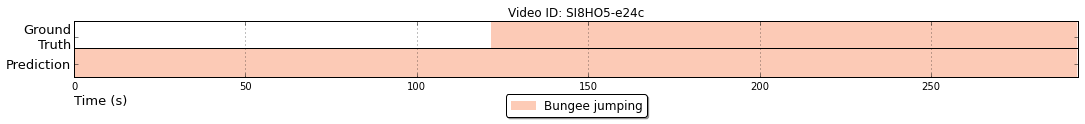
\includegraphics[width=1\linewidth]{img/results/activity_detection/activity_temporal_localization_12}
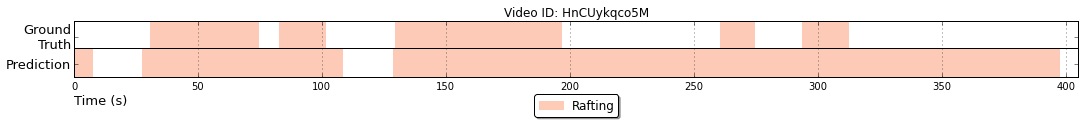
\includegraphics[width=1\linewidth]{img/results/activity_detection/activity_temporal_localization_13}
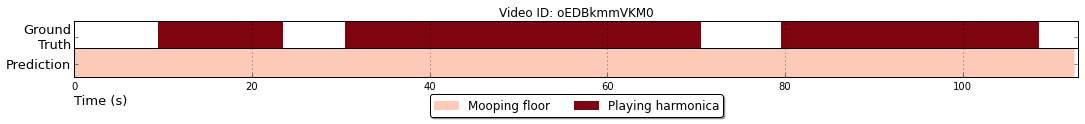
\includegraphics[width=1\linewidth]{img/results/activity_detection/activity_temporal_localization_14}
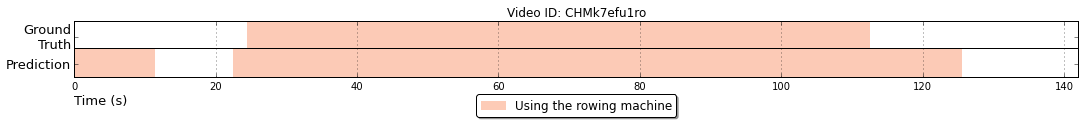
\includegraphics[width=1\linewidth]{img/results/activity_detection/activity_temporal_localization_15}
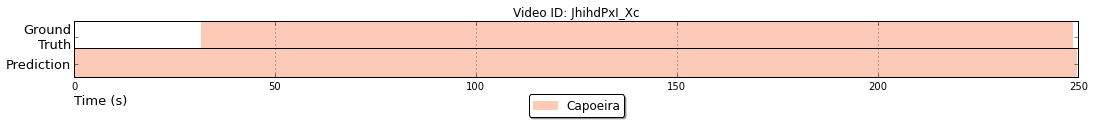
\includegraphics[width=1\linewidth]{img/results/activity_detection/activity_temporal_localization_16}
\includegraphics[width=1\linewidth]{img/results/activity_detection/activity_temporal_localization_17}
\includegraphics[width=1\linewidth]{img/results/activity_detection/activity_temporal_localization_18}
\includegraphics[width=1\linewidth]{img/results/activity_detection/activity_temporal_localization_19}
\includegraphics[width=1\linewidth]{img/results/activity_detection/activity_temporal_localization_20}
\includegraphics[width=1\linewidth]{img/results/activity_detection/activity_temporal_localization_21}
\includegraphics[width=1\linewidth]{img/results/activity_detection/activity_temporal_localization_22}
\includegraphics[width=1\linewidth]{img/results/activity_detection/activity_temporal_localization_23}
\end{center}
\caption{Temporal activity localization prediction done by the proposed neural network.}
\label{fig:results_visualization_detection_annex_1}
\end{figure}

\begin{figure}[H]
\begin{center}
\includegraphics[width=1\linewidth]{img/results/activity_detection/activity_temporal_localization_24}
\includegraphics[width=1\linewidth]{img/results/activity_detection/activity_temporal_localization_25}
\includegraphics[width=1\linewidth]{img/results/activity_detection/activity_temporal_localization_26}
\includegraphics[width=1\linewidth]{img/results/activity_detection/activity_temporal_localization_27}
\includegraphics[width=1\linewidth]{img/results/activity_detection/activity_temporal_localization_28}
\includegraphics[width=1\linewidth]{img/results/activity_detection/activity_temporal_localization_29}
\includegraphics[width=1\linewidth]{img/results/activity_detection/activity_temporal_localization_30}
\includegraphics[width=1\linewidth]{img/results/activity_detection/activity_temporal_localization_31}
\includegraphics[width=1\linewidth]{img/results/activity_detection/activity_temporal_localization_32}
\includegraphics[width=1\linewidth]{img/results/activity_detection/activity_temporal_localization_33}
\includegraphics[width=1\linewidth]{img/results/activity_detection/activity_temporal_localization_34}
\includegraphics[width=1\linewidth]{img/results/activity_detection/activity_temporal_localization_35}
\end{center}
\caption{Temporal activity localization prediction done by the proposed neural network.}
\label{fig:results_visualization_detection_annex_2}
\end{figure}

\chapter{Notebook Paper}

At the appendix there is the notebook submitted to the ActivityNet Challenge 2016 explaining the work done for to face the challenge.
\includepdf[pages={-}]{annex/upc_activitynet_challenge.pdf}



\bibliographystyle{plain}
\bibliography{ref/references}


\end{document}
